\documentclass[8pt]{beamer}

\usetheme{PSY9511}

\usepackage{emoji}
\usepackage{pgfplots}
\usepackage{pgfplotstable}
\usepackage{tikz}
\usepackage{transparent}
\usepackage{hyperref}

\hypersetup{
	colorlinks=false
}

\usepgfplotslibrary{fillbetween}
\usepgfplotslibrary{groupplots}

\usetikzlibrary{arrows.meta}
\usetikzlibrary{calc}
\usetikzlibrary{matrix}

\date{30.10.24}
\title{PSY2301: Psychology of judgement and decision making}
\subtitle{Artificial Intelligence and decision making}
\author{Esten H. Leonardsen}

\def\logoheight{1.2cm}
\def\logosep{0.5cm}

\colorlet{nodefill}{teal!20}
\colorlet{background}{gray!10}

\begin{document}

	\begin{frame}
		\maketitle
	\end{frame}

	\begin{frame}{Outline}
		\begin{enumerate}
			\item The history of artificial intelligence (AI).
			\item Terminology and concepts.
			\item How does AI make decisions?
			\item How can AI be used to support judgment and decision-making processes?
			\item How are decisions made by AIs perceived?
		\end{enumerate}
	\end{frame}

	\definecolor{activehistory}{HTML}{E71D36}
	\definecolor{passivehistory}{HTML}{939597}

	\section{The history of artificial intelligence}

	\newcommand{\imagenetplot}[1]{
		\begin{tikzpicture}
			\begin{axis}[
				ylabel={Error rate},
				xlabel={Year},
				xtick={2010, 2012, 2014, 2016, 2018, 2020},
				xticklabels={2010, 2012, 2014, 2016, 2018, 2020},
				ytick={0, 10, 20, 30},
				yticklabels={0\%, 10\%, 20\%, 30\%},
				ytick style={draw=none},
				ytick pos=left,
				xtick pos=bottom,
				ymajorgrids=true,
				ymax=29,
				ymin=0,
				xmin=2009,
				xmax=2021,
				width=8cm,
				height=5cm
			]
				\ifnum#1=0
					\addplot[mark=*, purple,thick] coordinates {
						(2010, 28.2)
						(2011, 25.8)
					};
				\fi
				\ifnum#1=1
					\addplot[mark=*, purple,thick] coordinates {
						(2010, 28.2)
						(2011, 25.8)
						(2012, 16.4)
					};
				\fi
				\ifnum#1>1
					\addplot[mark=*, purple,thick] coordinates {
						(2010, 28.2)
						(2011, 25.8)
						(2012, 16.4)
						(2013, 11.7)
						(2014, 7.3)
						(2015, 3.5)
						(2016, 3.0)
						(2017, 2.3)
						(2018, 1.8)
						(2019, 1.3)
						(2020, 0.9)
					};
				\fi

				\node[anchor=north, inner sep=5pt] at (axis cs: 2010, 28.2) {
					\small{28.2}
				};
				\node[anchor=north, inner sep=5pt] at (axis cs: 2011, 25.8) {
					\small{25.8}
				};

				\ifnum#1>0
					\node[anchor=north, inner sep=5pt] at (axis cs: 2012, 16.4) {
						\small{16.4}
					};

					\addplot[densely dotted] coordinates {
						(2011.5, 30)
						(2011.5, 0)
					};
				\fi
				\ifnum#1>1
					\node[anchor=north, inner sep=5pt] at (axis cs: 2013, 11.7) {
						\small{11.7}
					};
					\node[anchor=north, inner sep=5pt] at (axis cs: 2014, 7.3) {
						\small{7.3}
					};
					\node[anchor=north, inner sep=5pt] at (axis cs: 2015, 3.5) {
						\small{3.5}
					};
					\node[anchor=south, inner sep=5pt] at (axis cs: 2016, 3.0) {
						\small{3.0}
					};
					\node[anchor=south, inner sep=5pt] at (axis cs: 2017, 2.3) {
						\small{2.3}
					};
					\node[anchor=south, inner sep=5pt] at (axis cs: 2018, 1.8) {
						\small{1.8}
					};
					\node[anchor=south, inner sep=5pt] at (axis cs: 2019, 1.3) {
						\small{1.3}
					};
					\node[anchor=south, inner sep=5pt] at (axis cs: 2020, 0.9) {
						\small{\textbf{0.9}}
					};
				\fi
				\ifnum#1>2
					\addplot[dashed, red] coordinates {
						(2009, 5.1)
						(2021, 5.1)
					};

					\node[anchor=south east] at (axis cs: 2021, 5.1) {
						\textcolor{red}{\small{Human level}}
					};
				\fi
			\end{axis}
		\end{tikzpicture}
	}

	\newsavebox{\imagenetold}
	\sbox{\imagenetold}{
		\imagenetplot{0}
	}
	\newsavebox{\imagenetcnn}
	\sbox{\imagenetcnn}{
		\imagenetplot{1}
	}
	\newsavebox{\imagenetrecent}
	\sbox{\imagenetrecent}{
		\imagenetplot{2}
	}
	\newsavebox{\imagenethuman}
	\sbox{\imagenethuman}{
		\imagenetplot{3}
	}

	\begin{frame}{The history of artificial intelligence}
		\definecolor{activehistory}{HTML}{E71D36}
		\colorlet{passivehistory}{gray}

		\newcommand{\historynode}[4]{
			\pgfmathsetmacro{\ycoord}{ifthenelse(####3==1, 2.95, 2.55)}
			\pgfmathsetmacro{\anchorval}{ifthenelse(####3==1, "south", "north")}

			\node[
				circle,
				draw=####4,
				fill=####4
			] at (####1, 2.75) {};
			\node[
				anchor=\anchorval,
				baseline,
				text=####4,
				align=center,
				font=\small\linespread{0.9}\selectfont,
				inner sep=0pt,
				align=center
			] at (####1, \ycoord) {####2};
		}

		\newcommand{\activenode}[3]{
			\historynode{####1}{####2}{####3}{activehistory}
		}

		\newcommand{\passivenode}[3]{
			\historynode{####1}{####2}{####3}{passivehistory}
		}

		\newcommand{\conditionalreference}[6]{
			\visible<####1>{
				\node[font=\tiny\selectfont, text depth=0] at (0, -4.1) {
					\href{####2}{####3}, {####4}, \textit{####5}, ####6
				};
			}
		}

		\begin{tikzpicture}
			\node[] at (-5.25, 3.5) {};
			\node[] at (5.25, -4.2) {};

			\draw[very thick, passivehistory] (-4.75, 2.75)  -- (-3.6, 2.75) {};

			\visible<1-2>{
				\activenode{-3.6}{Turing\\test\\(1950)}{0}

				\node[
					inner sep=0pt,
					draw=black,
					label=below:{Alan Turing},
					anchor=west
				] at (-4.5, -1) {
					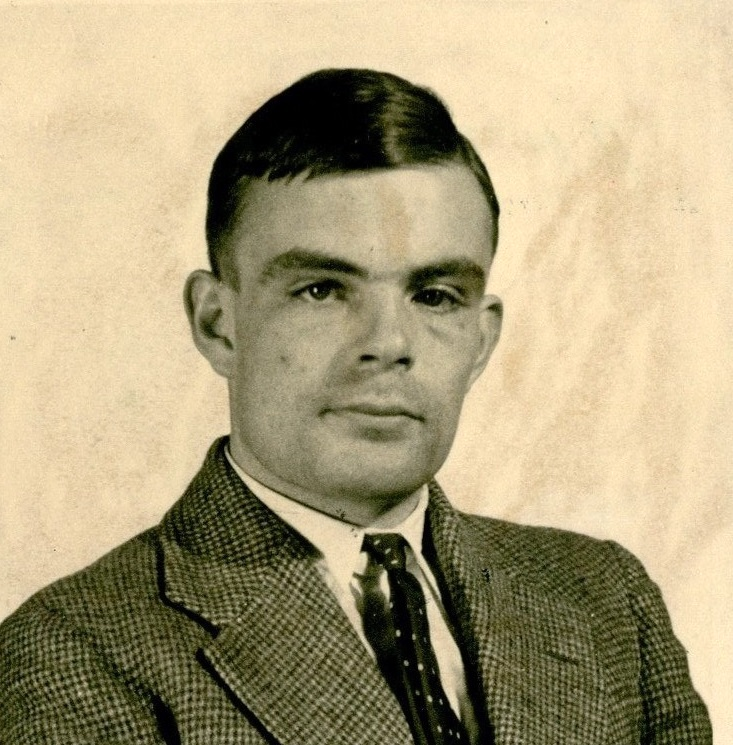
\includegraphics[width=3.5cm]{data/turing.jpeg}
				};
			}
			\visible<2>{
				\node[
					inner sep=0pt,
					draw=black,
					anchor=east
				] (patient) at (4.5, -1) {
					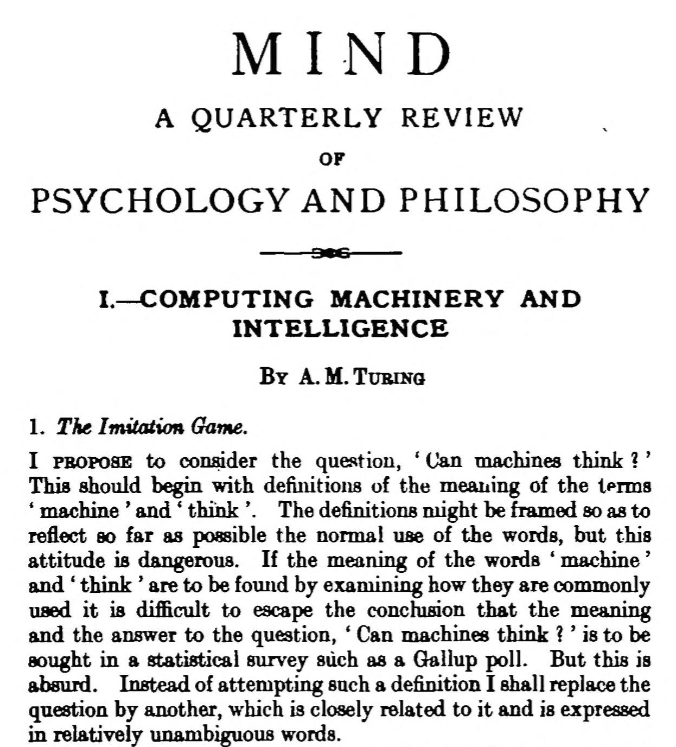
\includegraphics[width=4cm]{data/thinking.png}
				};
			}
			\conditionalreference{2}{https://link.springer.com/chapter/10.1007/978-1-4020-6710-5_3}{Computing Machinery and Intelligence}{A. M. Turing}{Mind}{1950}

			\visible<3->{
				\draw[very thick, gray] (-3.6, 2.75)  -- (-2.9, 2.75) {};
				\passivenode{-3.6}{Turing\\test\\(1950)}{0}
			}
			\visible<3-4>{
				\activenode{-2.9}{Dartmouth\\(1956)}{1}
			}
			\visible<3>{
				\node[inner sep=0pt] (patient) at (0, -1) {
					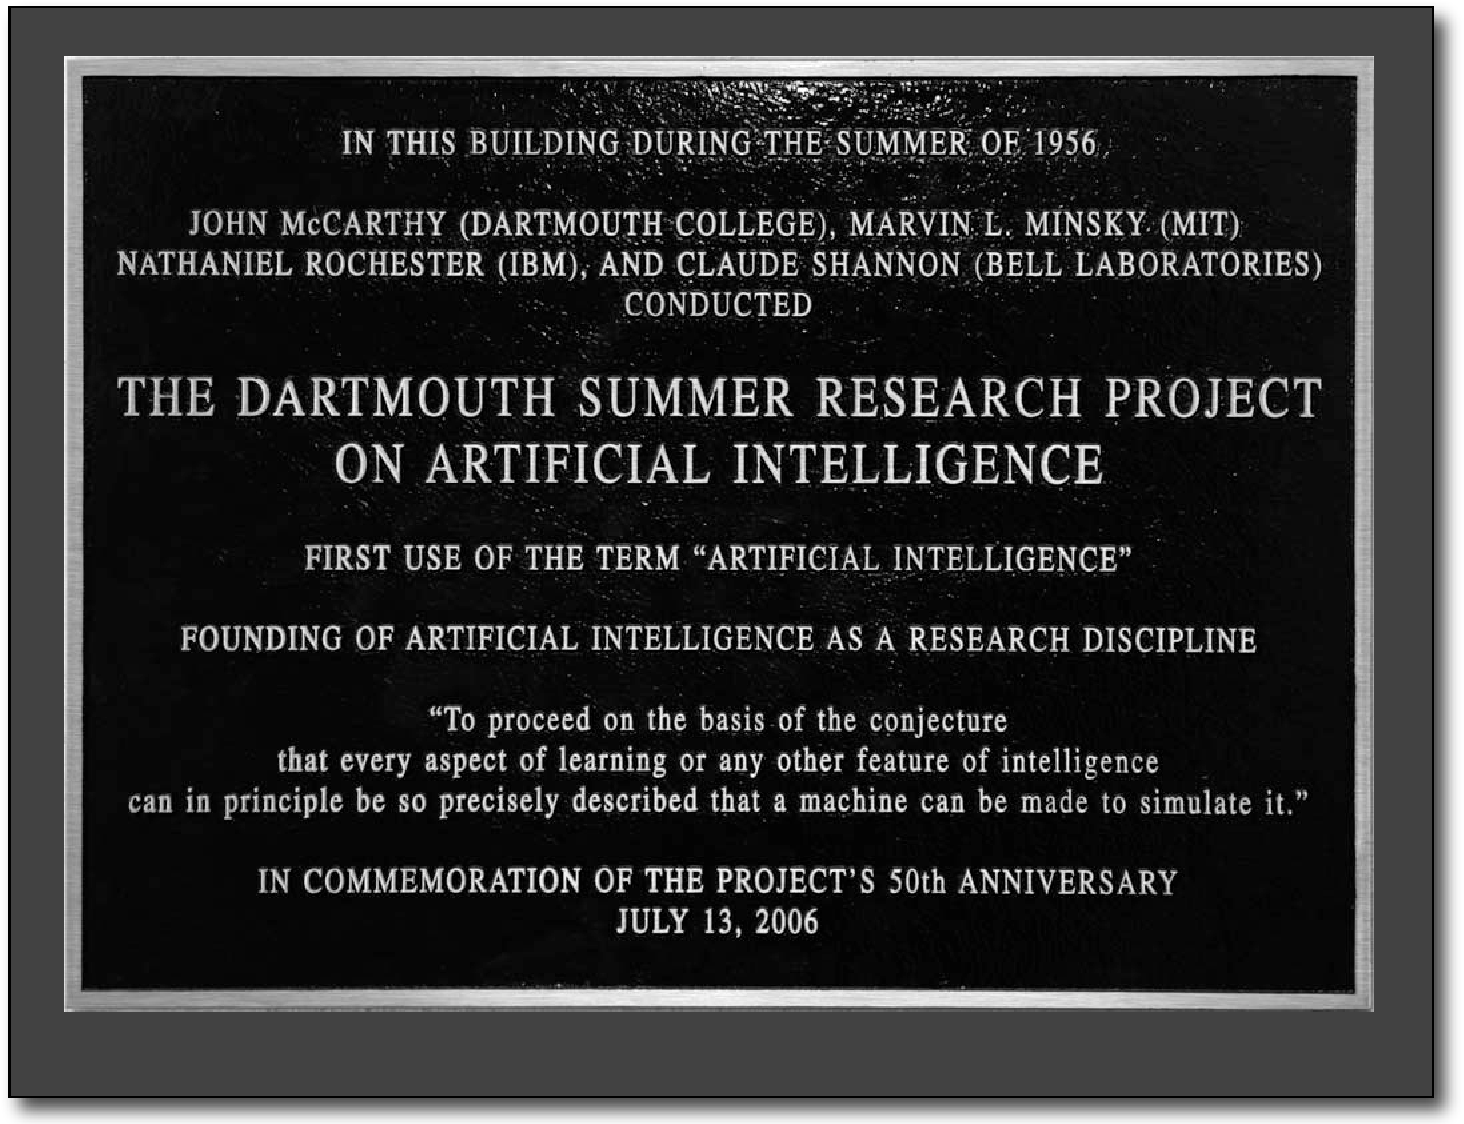
\includegraphics[width=6cm]{data/dartmouth.png}
				};
			}
			\visible<4>{
				\node[inner sep=0pt, align=center] (patient) at (0, -1) {
					"We propose that a 2-month, 10-man study of artificial intelligence\\
					be carried out [...]. An attempt will be made to find how to make\\
					machines use language, form abstractions and concepts, solve kinds\\
					of problems now reserved for humans, and improve themselves. We think\\
					that a significant advance can be made in [...] a summer."\\
					\textbf{- Proposal, Dartmouth summer school (1956)}
				};
			}
			\visible<5->{
				\passivenode{-2.9}{Dartmouth\\(1956)}{1}
				\draw[very thick, passivehistory] (-2.9, 2.75)  -- (-2.57, 2.75) {};
			}
			\visible<5-6>{
				\activenode{-2.57}{Perceptron\vphantom{i}\\(1958)}{0}

				\node[draw=black, inner sep=5pt, fill=white] (patient) at (-2, -1) {
					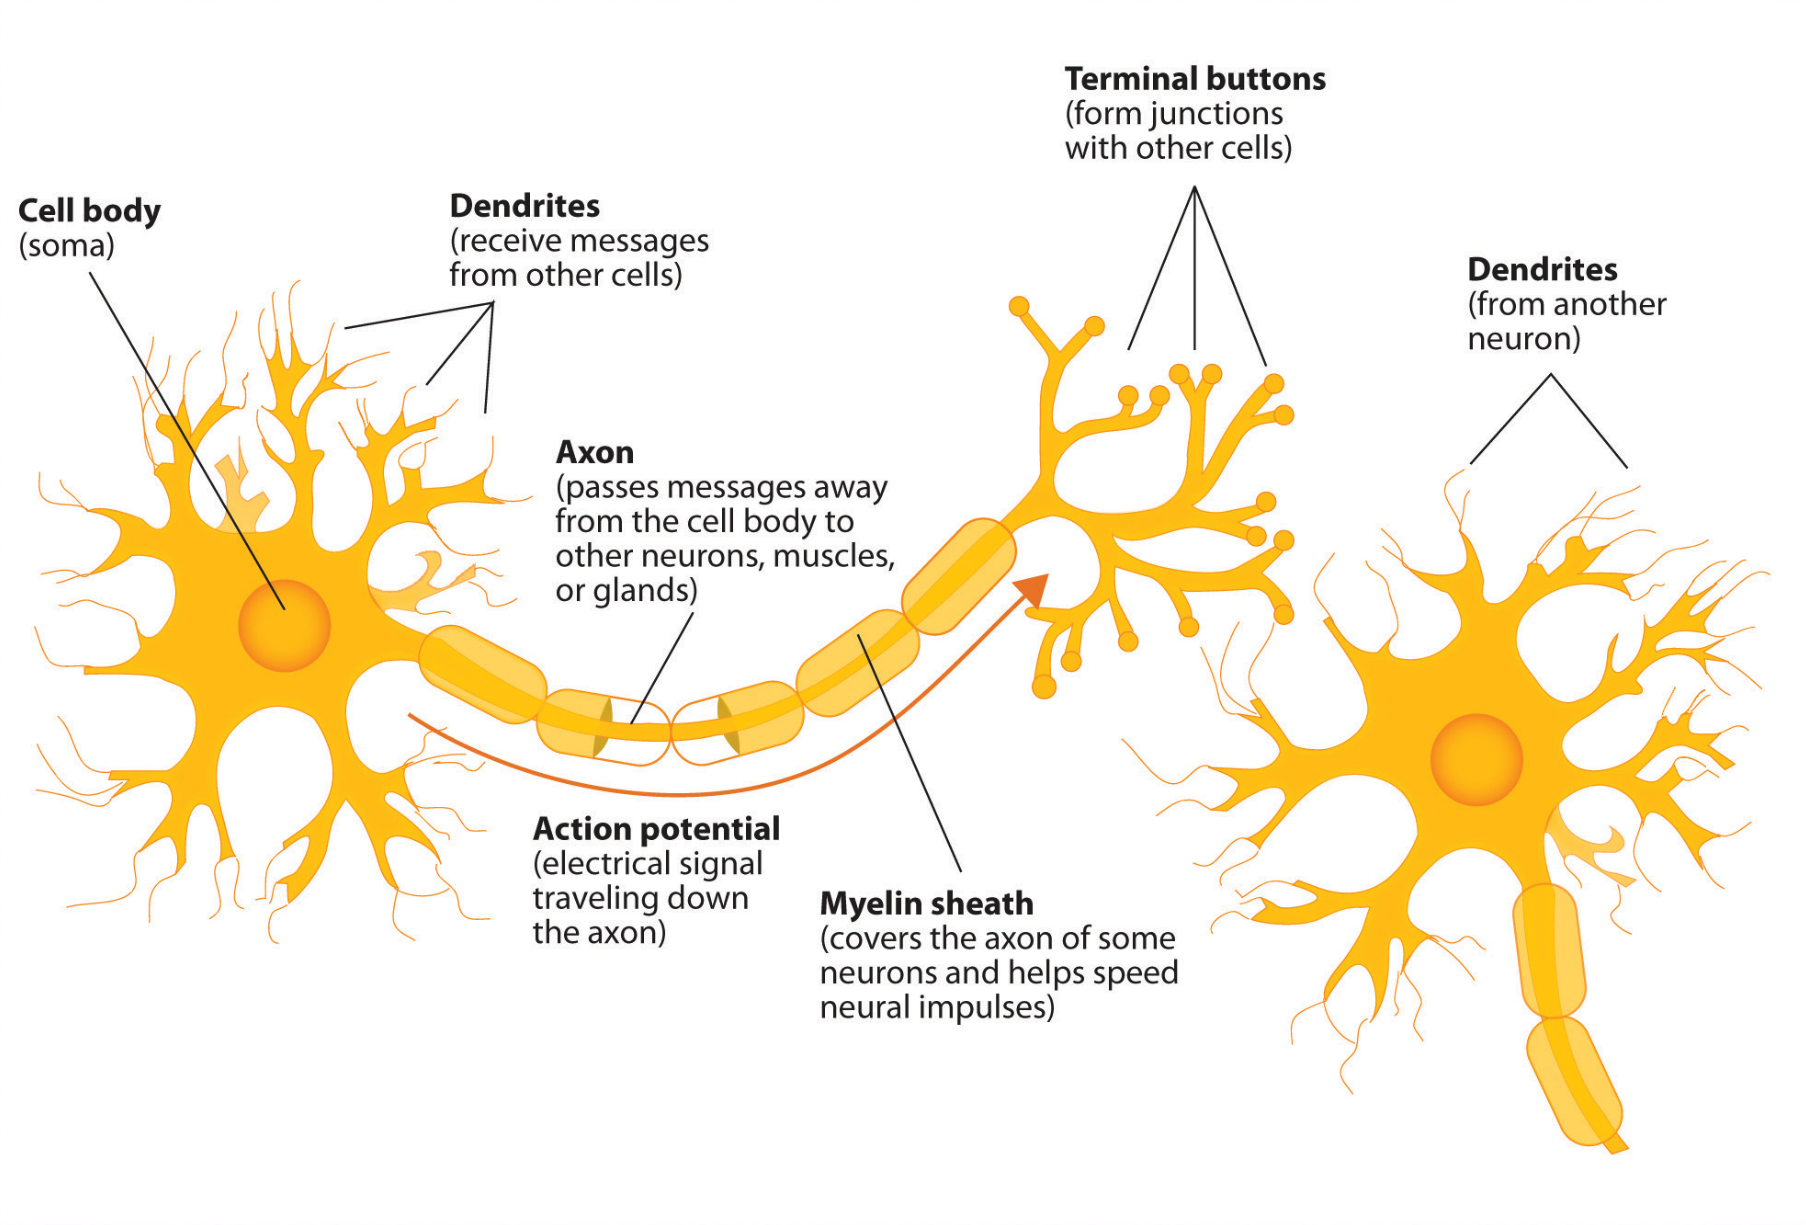
\includegraphics[width=4cm]{data/neuron.png}
				};
			}

			\conditionalreference{5}{https://opentextbc.ca/introductiontopsychology/chapter/3-1-the-neuron-is-the-building-block-of-the-nervous-system/}{The neuron is the building block of the nervous system}{Stangor, C. and Walinga, J}{Introduction to psychology}{2024}

			\visible<6>{
				\node[circle, draw=black, fill=nodefill, inner sep=2pt, text depth=0] (node) at (3, -1) {+};

				\node[] (x0) at ($ (node) - (1.25, -1) $) {$\mathrm{input}_0$};
				\node[] (x1) at ($ (node) - (1.25, 0) $) {$\mathrm{input}_1$};
				\node[] (x2) at ($ (node) - (1.25, 1) $) {$\mathrm{input}_2$};

				\node[align=center] (out) at ($ (node) + (1.25, 0) $) {$\mathrm{output}$\\$\mathrm{(0/1)}$};

				\draw[-Latex] (x0) -- (node) node [midway, above] {\small{$w_0$}};
				\draw[-Latex] (x1) -- (node) node [midway, below] {\small{$w_1$}};;
				\draw[-Latex] (x2) -- (node) node [midway, below] {\small{$w_2$}};;
				\draw[-Latex] (node) -- (out);
			}
			\visible<7->{
				\passivenode{-2.57}{Perceptron\vphantom{i}\\(1958)}{0}
				\draw[very thick, passivehistory] (-2.57, 2.75)  -- (-1.97, 2.75) {};
			}
			\visible<7>{
				\activenode{-1.97}{Eliza\\(1964)}{1}

				\node[draw=black, inner sep=5pt, fill=white] (patient) at (0, -1) {
					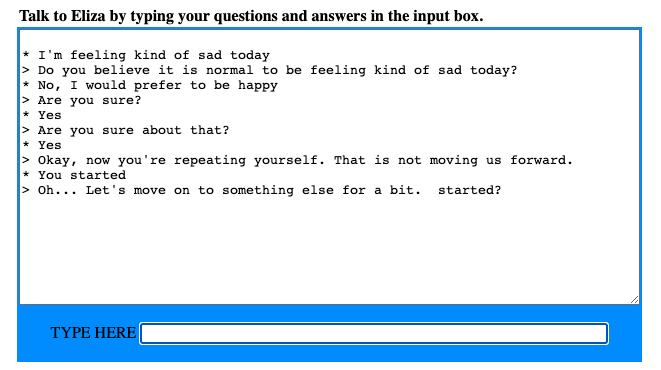
\includegraphics[width=7cm]{data/eliza.png}
				};
				\node[font=\tiny\selectfont, text depth=0] at (0, -4.1) {
					\href{https://web.njit.edu/~ronkowit/eliza.html}{ELIZA: a very basic Rogerian psychotherapist chatbot}
				};
			}

			\visible<8->{
				\passivenode{-1.97}{Eliza\\(1964)}{1}
				\draw[very thick, passivehistory] (-1.97, 2.75)  -- (-0.12, 2.75) {};
			}

			\visible<8-9>{
				\activenode{-0.12}{Expert\vphantom{i}\\systems\\(1980s)}{0}
			}
			\visible<8>{
				\node[] (patient) at (0, 0.5) {
					\Huge{\emoji{face-with-medical-mask}}
				};
				\node[draw=black, align=center ] (interface) at ($ (patient.south) - (0, 0.8) $) {
					User interface
				};

				\node[draw=black] (inference) at ($ (interface.south) - (0, 0.5) $) {
					Inference engine
				};
				\node[draw=black] (database) at ($ (inference.south) - (0, 0.5) $) {
					Knowledge database
				};
				\node[] (doctor) at ($ (database.south) - (0, 0.9) $) {
					\Huge{\emoji{woman-scientist}}
				};

				\draw[-Latex] ($ (patient.south) - (0.1, 0) $) -- ($ (interface.north) - (0.1, 0) $);
				\draw[Latex-] ($ (patient.south) + (0.1, 0) $) -- ($ (interface.north) + (0.1, 0) $);
				\draw[-Latex] ($ (interface.south) - (0.1, 0) $) -- ($ (inference.north) - (0.1, 0) $);
				\draw[Latex-] ($ (interface.south) + (0.1, 0) $) -- ($ (inference.north) + (0.1, 0) $);
				\draw[Latex-] (inference.south) -- (database.north);
				\draw[Latex-, dashed] (database.south) -- (doctor.north);

				\draw[densely dotted] ($ (interface.north west) + (-1.3, 0.1) $) rectangle ($ (database.south east) + (1, -0.1) $);

				\node[anchor=north east] at ($ (patient.south) - (0.1, 0.05) $) {\small{Query}};
				\node[anchor=north west] at ($ (patient.south) - (-0.1, 0.05) $) {\small{Response}};
			}
			\visible<9>{
				\node[inner sep=0pt, draw=black] (patient) at (0, -1) {
					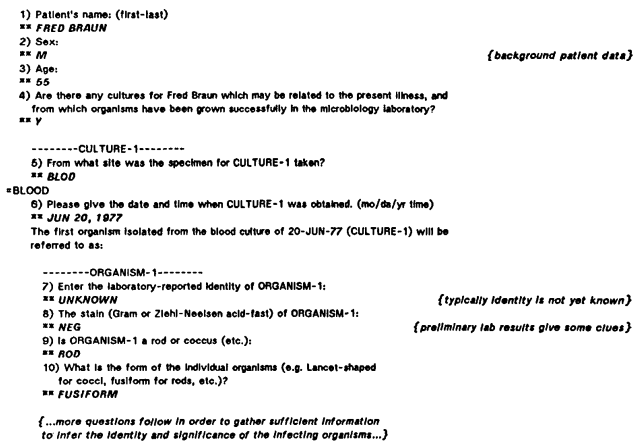
\includegraphics[width=6.5cm]{data/mycin.png}
				};
			}
			\conditionalreference{9}{https://www.sciencedirect.com/science/article/pii/S0020737378800492}{MYCIN}{William van Melle}{International Journal of Man-Machine Studies}{1978}

			\visible<10->{
				\passivenode{-0.12}{Expert\vphantom{i}\\systems\\(1980s)}{0}
				\draw[very thick, passivehistory] (-0.12, 2.75)  -- (0.57, 2.75) {};
			}
			\visible<10-14>{
				\activenode{0.57}{Artificial neural networks\\(1986)}{1}
			}
			\visible<10>{
				\node[inner sep=0pt, minimum size=0.4cm, draw=black, circle, fill=nodefill] (n00) at (0, -1.5) {};

				\node[] (x0) at ($ (n00) - (1.25, 0.75) $) {$\mathrm{input}_0$};
				\node[] (x1) at ($ (n00) - (1.25, 0) $) {$\mathrm{input}_1$};
				\node[] (x2) at ($ (n00) - (1.25, -0.75) $) {$\mathrm{input}_2$};

				\node[] (out) at ($ (n00) + (1.25, 0) $) {$\mathrm{output}$};

				\draw[-] (x0.east) -- (n00);
				\draw[-] (x1.east) -- (n00);
				\draw[-] (x2.east) -- (n00);

				\draw[->] (n00) -- (out);
			}
			\visible<11,13>{
				\node[] (x0) at (-2.75, -0.75) {$\mathrm{input}_0$};
				\node[] (x1) at ($ (x0) - (0, 0.75) $) {$\mathrm{input}_1$};
				\node[] (x2) at ($ (x0) - (0, 1.5) $) {$\mathrm{input}_2$};

				\node[inner sep=0pt, minimum size=0.4cm, draw=black, circle, fill=nodefill] (n00) at ($ (x0) + (1.25, 0.25) $) {};
				\node[inner sep=0pt, minimum size=0.4cm, draw=black, circle, fill=nodefill] (n01) at ($ (x0) + (1.25, -0.25) $) {};
				\node[inner sep=0pt, minimum size=0.4cm, draw=black, circle, fill=nodefill] (n02) at ($ (x0) + (1.25, -0.75) $) {};
				\node[inner sep=0pt, minimum size=0.4cm, draw=black, circle, fill=nodefill] (n03) at ($ (x0) + (1.25, -1.25) $) {};
				\node[inner sep=0pt, minimum size=0.4cm, draw=black, circle, fill=nodefill] (n04) at ($ (x0) + (1.25, -1.75) $) {};

				\node[inner sep=0pt, minimum size=0.4cm, draw=black, circle, fill=nodefill] (n10) at ($ (x0) + (2, 0) $) {};
				\node[inner sep=0pt, minimum size=0.4cm, draw=black, circle, fill=nodefill] (n11) at ($ (x0) + (2, -0.5) $) {};
				\node[inner sep=0pt, minimum size=0.4cm, draw=black, circle, fill=nodefill] (n12) at ($ (x0) + (2, -1) $) {};
				\node[inner sep=0pt, minimum size=0.4cm, draw=black, circle, fill=nodefill] (n13) at ($ (x0) + (2, -1.5) $) {};

				\node[inner sep=0pt, minimum size=0.4cm, draw=black, circle, fill=nodefill] (n20) at ($ (x0) + (2.75, -0.25) $) {};
				\node[inner sep=0pt, minimum size=0.4cm, draw=black, circle, fill=nodefill] (n21) at ($ (x0) + (2.75, -0.75) $) {};
				\node[inner sep=0pt, minimum size=0.4cm, draw=black, circle, fill=nodefill] (n22) at ($ (x0) + (2.75, -1.25) $) {};

				\node[inner sep=0pt, minimum size=0.4cm, draw=black, circle, fill=nodefill] (n30) at ($ (x0) + (3.5, -0.5) $) {};
				\node[inner sep=0pt, minimum size=0.4cm, draw=black, circle, fill=nodefill] (n31) at ($ (x0) + (3.5, -1) $) {};

				\node[inner sep=0pt, minimum size=0.4cm, draw=black, circle, fill=nodefill, text depth=0] (n40) at ($ (x0) + (4.25, -0.75) $) {};
				\node[] (out) at ($ (x0) + (5.5, -0.75) $) {$\mathrm{output}$};
			}
			\visible<11>{
				\draw[-] (x0.east) -- (n00);
				\draw[-] (x0.east) -- (n01);
				\draw[-] (x0.east) -- (n02);
				\draw[-] (x0.east) -- (n03);
				\draw[-] (x0.east) -- (n04);
				\draw[-] (x1.east) -- (n00);
				\draw[-] (x1.east) -- (n01);
				\draw[-] (x1.east) -- (n02);
				\draw[-] (x1.east) -- (n03);
				\draw[-] (x1.east) -- (n04);
				\draw[-] (x2.east) -- (n00);
				\draw[-] (x2.east) -- (n01);
				\draw[-] (x2.east) -- (n02);
				\draw[-] (x2.east) -- (n03);
				\draw[-] (x2.east) -- (n04);

				\draw[-] (n00) -- (n10);
				\draw[-] (n00) -- (n11);
				\draw[-] (n00) -- (n12);
				\draw[-] (n00) -- (n13);
				\draw[-] (n01) -- (n10);
				\draw[-] (n01) -- (n11);
				\draw[-] (n01) -- (n12);
				\draw[-] (n01) -- (n13);
				\draw[-] (n02) -- (n10);
				\draw[-] (n02) -- (n11);
				\draw[-] (n02) -- (n12);
				\draw[-] (n02) -- (n13);
				\draw[-] (n03) -- (n10);
				\draw[-] (n03) -- (n11);
				\draw[-] (n03) -- (n12);
				\draw[-] (n03) -- (n13);
				\draw[-] (n04) -- (n10);
				\draw[-] (n04) -- (n11);
				\draw[-] (n04) -- (n12);
				\draw[-] (n04) -- (n13);

				\draw[-] (n10) -- (n20);
				\draw[-] (n10) -- (n21);
				\draw[-] (n10) -- (n22);
				\draw[-] (n11) -- (n20);
				\draw[-] (n11) -- (n21);
				\draw[-] (n11) -- (n22);
				\draw[-] (n12) -- (n20);
				\draw[-] (n12) -- (n21);
				\draw[-] (n12) -- (n22);
				\draw[-] (n13) -- (n20);
				\draw[-] (n13) -- (n21);
				\draw[-] (n13) -- (n22);

				\draw[-] (n20) -- (n30);
				\draw[-] (n20) -- (n31);
				\draw[-] (n21) -- (n30);
				\draw[-] (n21) -- (n31);
				\draw[-] (n22) -- (n30);
				\draw[-] (n22) -- (n31);

				\draw[-] (n30) -- (n40);
				\draw[-] (n31) -- (n40);

				\draw[->] (n40) -- (out);
			}
			\visible<13>{
				\draw[-] (x0.east) -- (n00);
				\draw[-] (x0.east) -- (n01);
				\draw[-] (x0.east) -- (n02);
				\draw[-] (x0.east) -- (n03);
				\draw[-] (x0.east) -- (n04);
				\draw[-] (x1.east) -- (n00);
				\draw[-] (x1.east) -- (n01);
				\draw[-] (x1.east) -- (n02);
				\draw[-] (x1.east) -- (n03);
				\draw[-] (x1.east) -- (n04);
				\draw[-] (x2.east) -- (n00);
				\draw[-] (x2.east) -- (n01);
				\draw[-] (x2.east) -- (n02);
				\draw[-] (x2.east) -- (n03);
				\draw[-] (x2.east) -- (n04);

				\draw[Latex-, red] (n00) -- (n10);
				\draw[Latex-, red] (n00) -- (n11);
				\draw[Latex-, red] (n00) -- (n12);
				\draw[Latex-, red] (n00) -- (n13);
				\draw[Latex-, red] (n01) -- (n10);
				\draw[Latex-, red] (n01) -- (n11);
				\draw[Latex-, red] (n01) -- (n12);
				\draw[Latex-, red] (n01) -- (n13);
				\draw[Latex-, red] (n02) -- (n10);
				\draw[Latex-, red] (n02) -- (n11);
				\draw[Latex-, red] (n02) -- (n12);
				\draw[Latex-, red] (n02) -- (n13);
				\draw[Latex-, red] (n03) -- (n10);
				\draw[Latex-, red] (n03) -- (n11);
				\draw[Latex-, red] (n03) -- (n12);
				\draw[Latex-, red] (n03) -- (n13);
				\draw[Latex-, red] (n04) -- (n10);
				\draw[Latex-, red] (n04) -- (n11);
				\draw[Latex-, red] (n04) -- (n12);
				\draw[Latex-, red] (n04) -- (n13);

				\draw[Latex-, red] (n10) -- (n20);
				\draw[Latex-, red] (n10) -- (n21);
				\draw[Latex-, red] (n10) -- (n22);
				\draw[Latex-, red] (n11) -- (n20);
				\draw[Latex-, red] (n11) -- (n21);
				\draw[Latex-, red] (n11) -- (n22);
				\draw[Latex-, red] (n12) -- (n20);
				\draw[Latex-, red] (n12) -- (n21);
				\draw[Latex-, red] (n12) -- (n22);
				\draw[Latex-, red] (n13) -- (n20);
				\draw[Latex-, red] (n13) -- (n21);
				\draw[Latex-, red] (n13) -- (n22);

				\draw[Latex-, red] (n20) -- (n30);
				\draw[Latex-, red] (n20) -- (n31);
				\draw[Latex-, red] (n21) -- (n30);
				\draw[Latex-, red] (n21) -- (n31);
				\draw[Latex-, red] (n22) -- (n30);
				\draw[Latex-, red] (n22) -- (n31);

				\draw[Latex-, red] (n30) -- (n40);
				\draw[Latex-, red] (n31) -- (n40);

				\draw[Latex-, red] (n40) -- (out);
			}
			\visible<12,14>{
				\node[inner sep=0pt, draw=black] (backprop) at (0, -1) {
					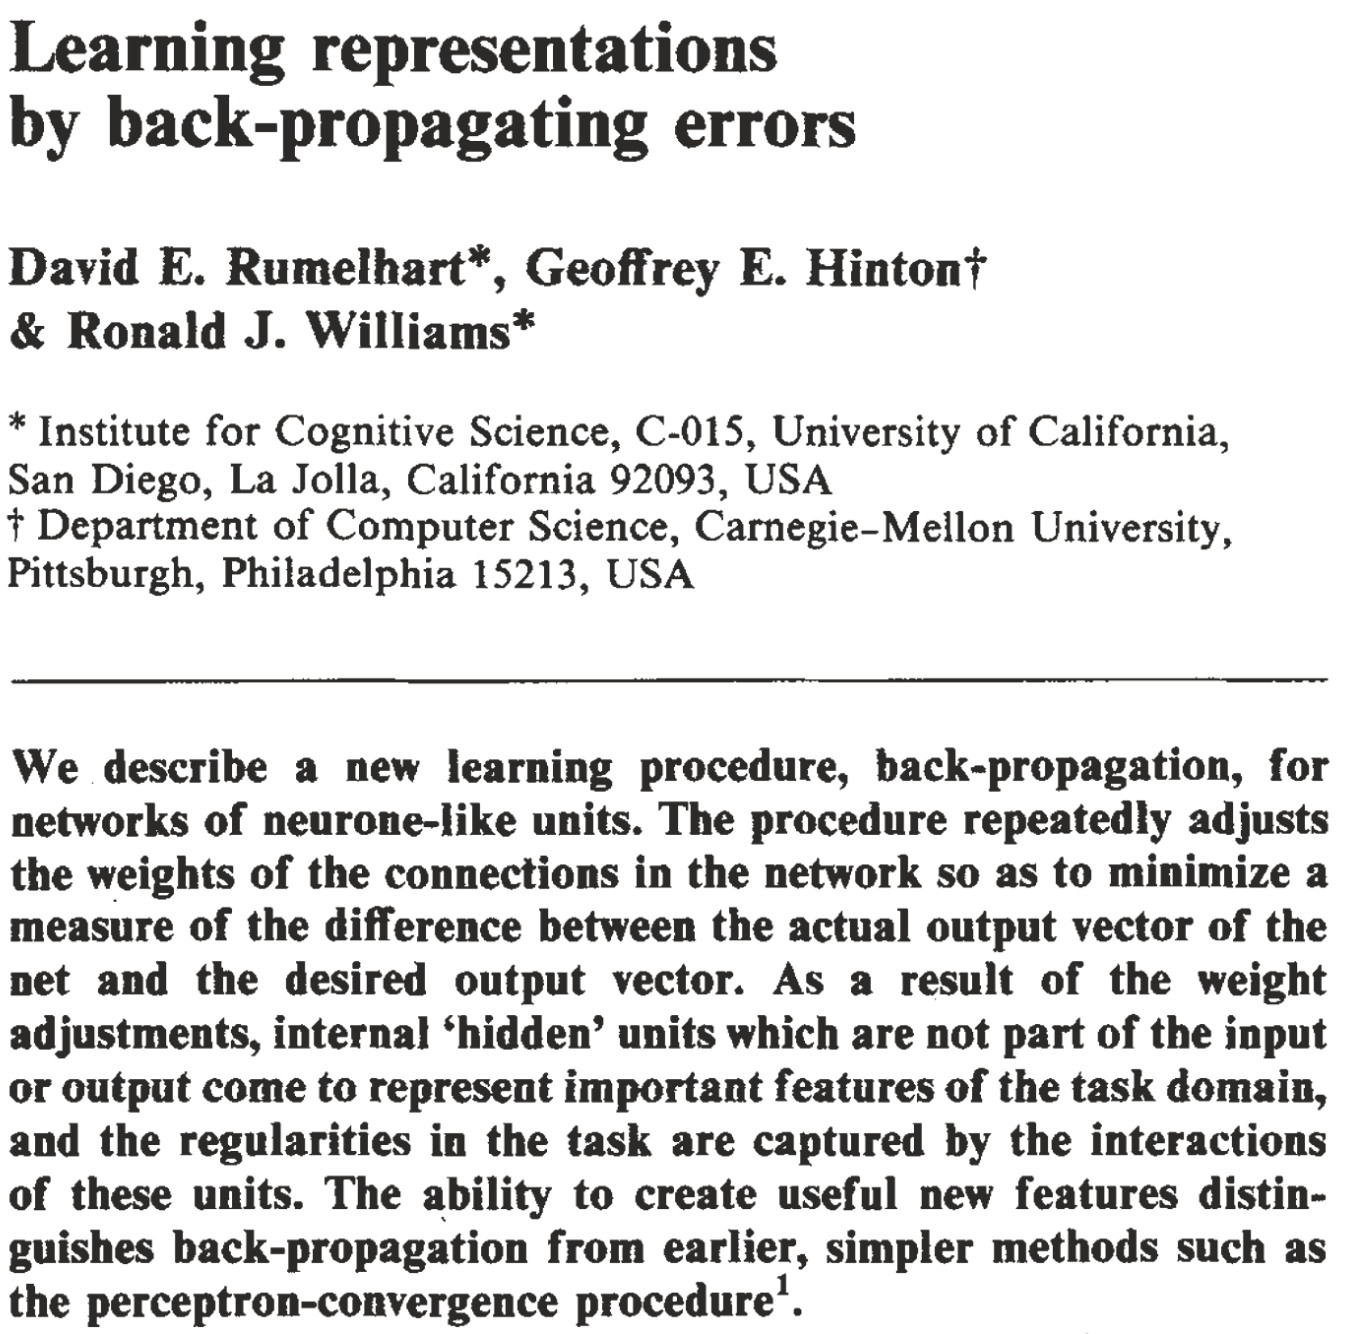
\includegraphics[width=5cm]{data/backprop.png}
				};
			}
			\conditionalreference{12}{https://www.nature.com/articles/323533a0}{Learning representations by back-propagating errors}{Rumelhart, D. et al.}{Nature}{1986}

			\visible<14>{
				\draw[red, thick] ($ (backprop.north) + (-0.55, -1.1) $) -- ($ (backprop.north) + (1.07, -1.1) $);
			}
			\visible<15->{
				\passivenode{0.57}{Artificial neural networks\\(1986)}{1}
				\draw[very thick, passivehistory] (0.57, 2.75)  -- (2.55, 2.75) {};
			}
			\visible<15>{
				\activenode{2.55}{Deep blue\vphantom{i}\\(1997)}{0}

				\node[inner sep=0pt, draw=black, label=below:{\small{DALL-E: "A robot playing chess"}}] (img) at (-2.25, -1) {
					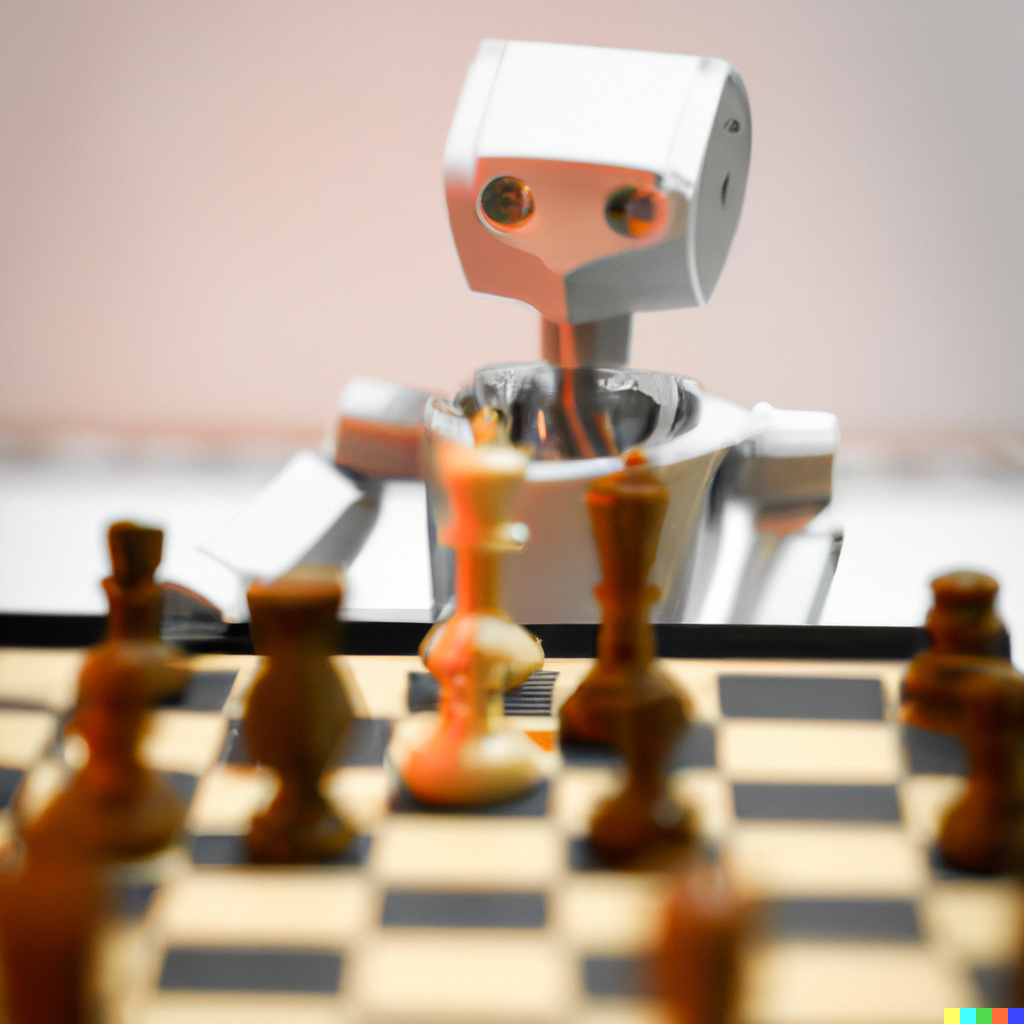
\includegraphics[width=4cm]{data/chess.png}
				};
				\node[anchor=north west, align=left] at ($ (img.north east)  + (0.1, 0) $) {
					\bullet\hspace{0.1cm}IBMs Deep Blue became the first\\ computer to beat the reigning human\\ world champion in chess.\\
					\bullet\hspace{0.1cm}Deep blue won with 3\textonehalf { }points to\\ Garry Kasparovs 2\textonehalf{ } after six matches.\\
					\bullet\hspace{0.1cm}Kasparov famously stated that\\"Deep Blue was intelligent the way your\\programmable alarm clock is intelligent."\\
				};
			}
			\visible<16->{
				\passivenode{2.55}{Deep blue\vphantom{i}\\(1997)}{0}
				\draw[very thick, passivehistory] (2.55, 2.75)  -- (4.29, 2.75) {};
			}
			\visible<16-21>{
				\activenode{4.29}{Deep learning\\(2012)}{1}
			}
			\visible<16-17>{
				\node[inner sep=0pt, label=below:\small{Cat}] (img3) at (0, -1) {
					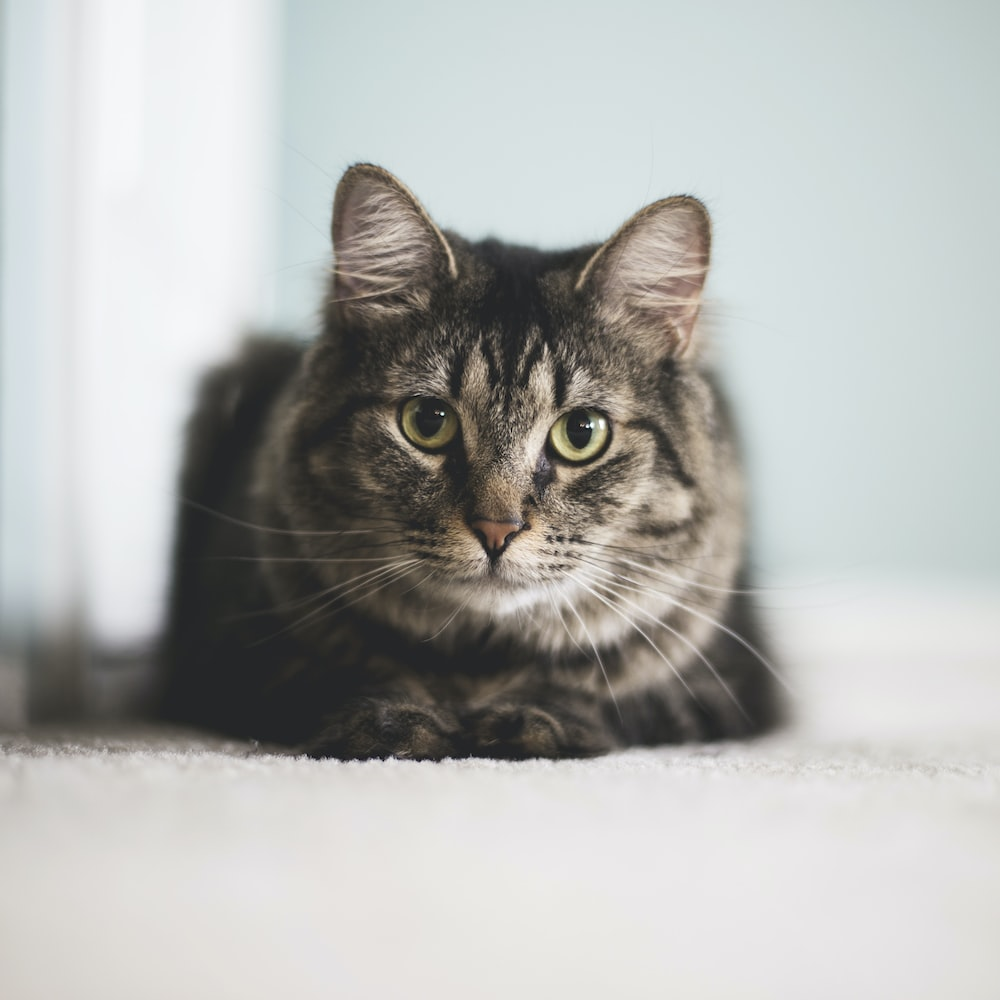
\includegraphics[width=1.5cm]{data/cat.jpeg}
				};
			}
			\visible<17>{
				\node[inner sep=0pt, label=below:\small{Airplane}, anchor=west] (img4) at ($ (img3.east) + (0.1, 0) $) {
					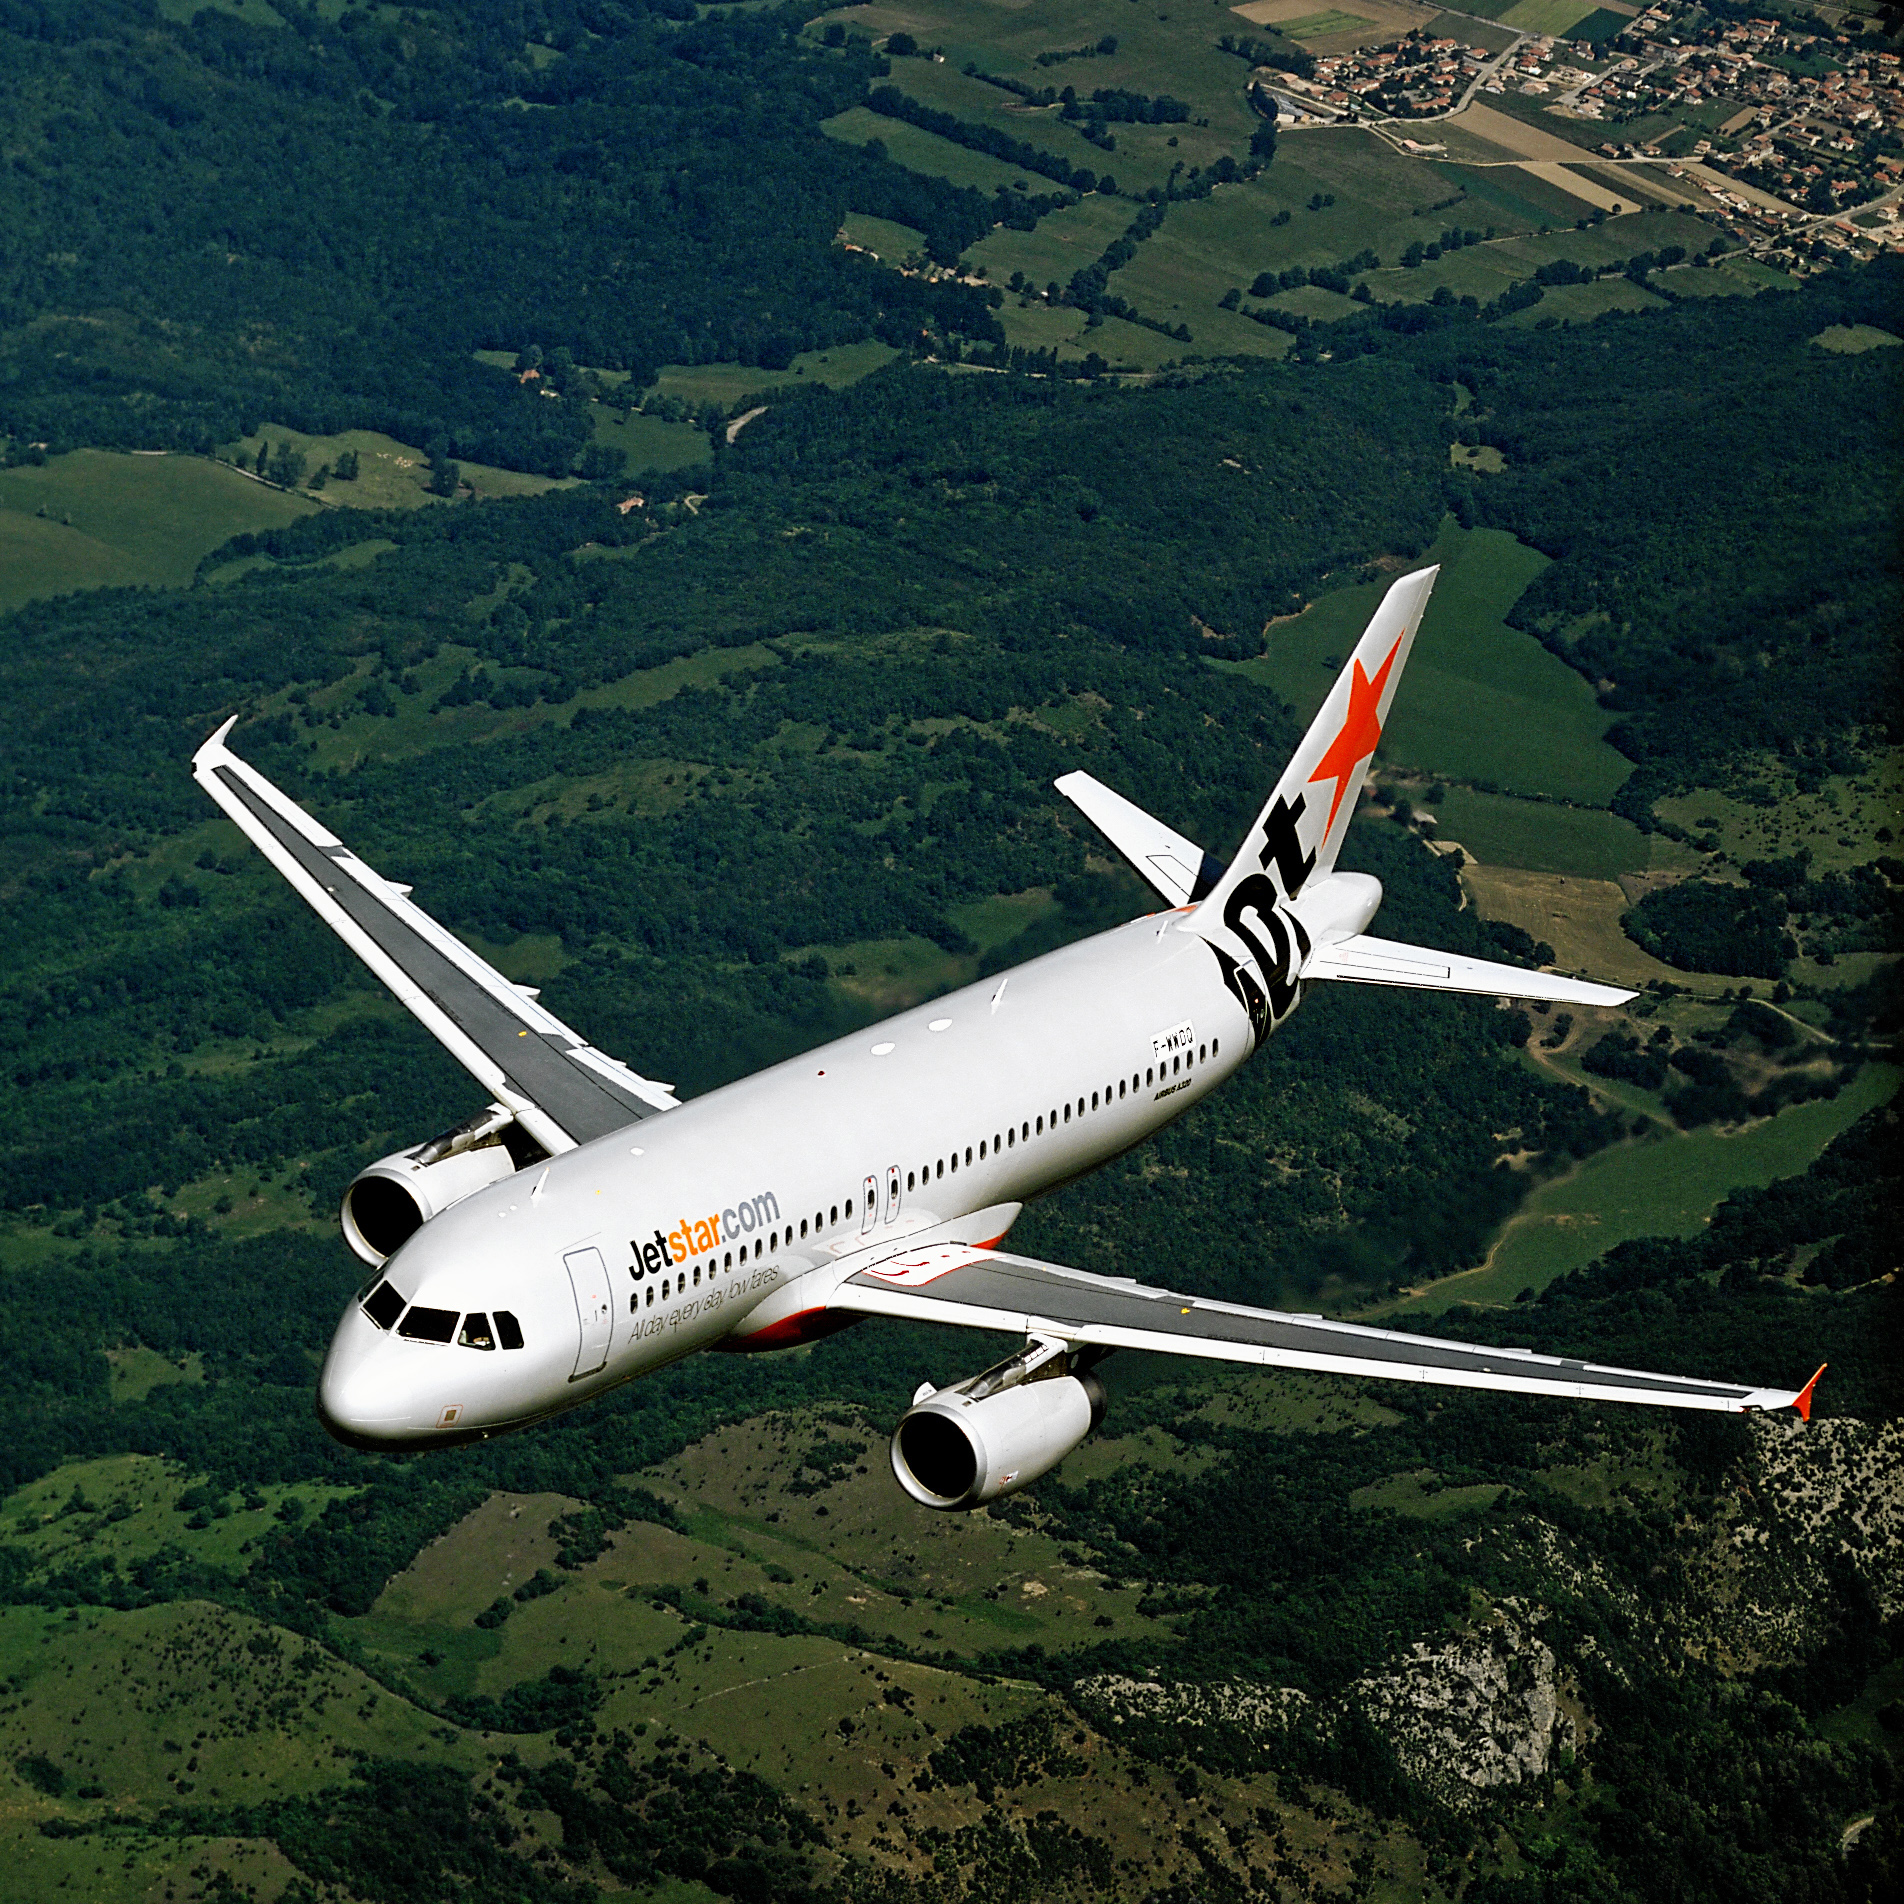
\includegraphics[width=1.5cm]{data/airplane.jpeg}
				};
				\node[inner sep=0pt, label=below:\small{Shark}, anchor=west] (img5) at ($ (img4.east) + (0.1, 0) $) {
					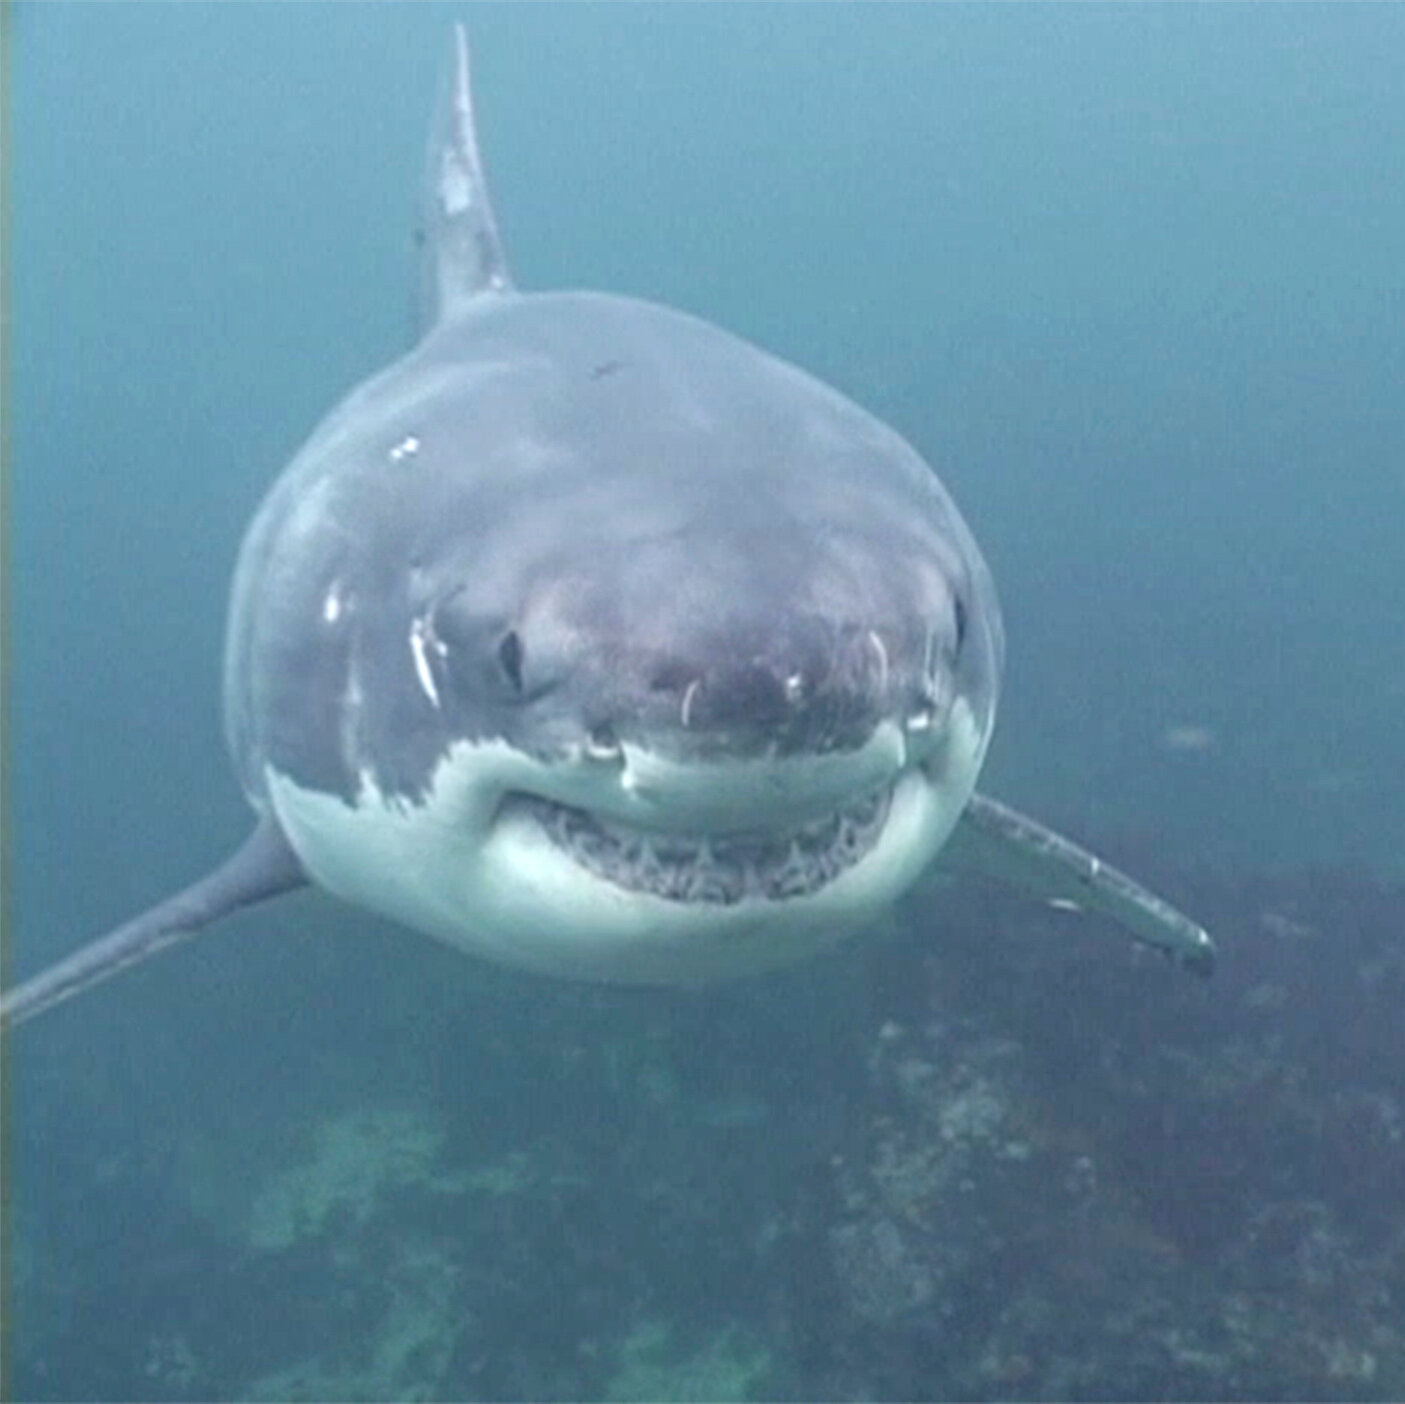
\includegraphics[width=1.5cm]{data/shark.jpeg}
				};
				\node[inner sep=0pt, label=below:\small{Ladybug}, anchor=east] (img2) at ($ (img3.west) - (0.1, 0) $) {
					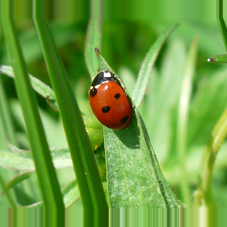
\includegraphics[width=1.5cm]{data/ladybug.png}
				};
				\node[inner sep=0pt, label=below:\small{Sunflower}, anchor=east] (img1) at ($ (img2.west) - (0.1, 0) $) {
					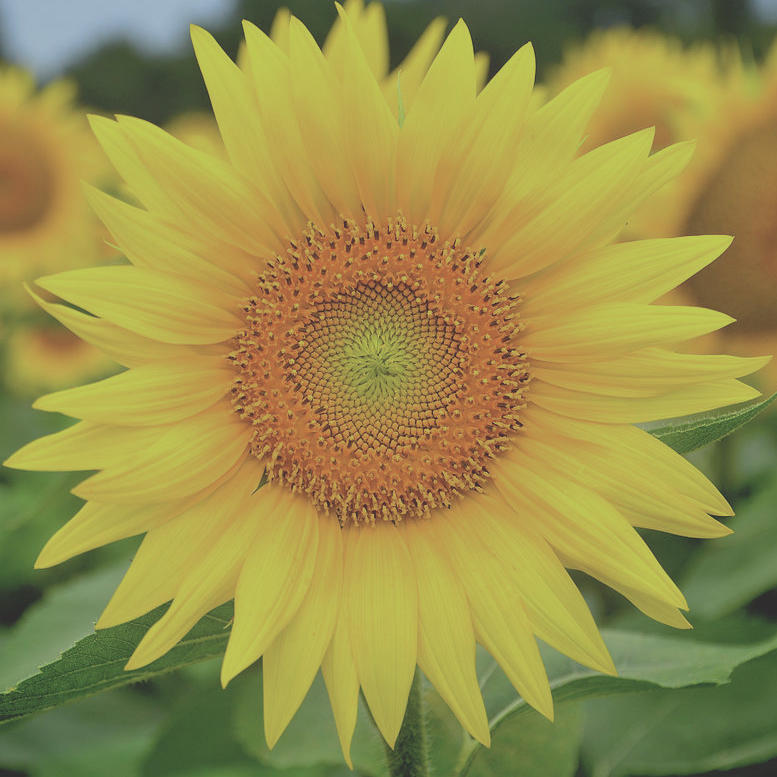
\includegraphics[width=1.5cm]{data/sunflower.jpeg}
				};
				\node[] at (0, -2.5) {
					ImageNet: $\sim$14m images, $\sim$22k categories
				};
			}
			\visible<18>{
				\node[] at (0, -1) {
					\usebox{\imagenetold}
				};
			}
			\visible<19>{
				\node[] at (0, -1) {
					\usebox{\imagenetcnn}
				};
			}
			\visible<20>{
				\node[] at (0, -1) {
					\usebox{\imagenetrecent}
				};
			}
			\visible<21>{
				\node[] at (0, -1) {
					\usebox{\imagenethuman}
				};
			}
			\visible<22>{
				\passivenode{4.29}{Deep learning\\(2012)}{1}
				\draw[very thick, passivehistory] (4.29, 2.75)  -- (5.45, 2.75) {};
				\activenode{5.45}{ChatGPT\\(2022)}{0}

				\node[inner sep=0pt, draw=black] at (0, -1.25) {
					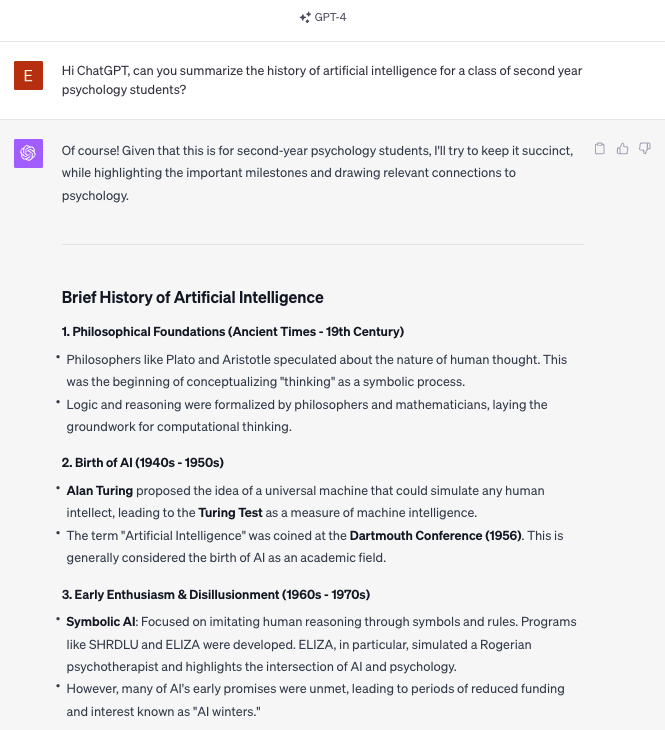
\includegraphics[width=4.5cm]{data/chatgpt.png}
				};
			}
		\end{tikzpicture}
	\end{frame}

	\section{Terminology and concepts}

	\begin{frame}{Terminology and concepts: Taxonomy}
		\centering
		\vfill
		\begin{tikzpicture}
			\node[circle, fill=blue!60, minimum size=6cm] (ai) at (0, 0) {};
			\node[text=white, anchor=north] at ($ (ai.north) - (0, 0.3) $) {\textbf{Artificial intelligence}};

			\visible<1>{
				\node[anchor=north west, align=left, font=\small] (ai-text) at ($ (ai.north) + (3.5, 0.2) $) {\textbf{Artificial intelligence:}\\Machines that solve tasks\\requiring intelligence};
			}
			\visible<2->{
				\node[anchor=north west, align=left, font=\small, text=gray!40] (ai-text) at ($ (ai.north) + (3.5, 0.2) $) {\textbf{Artificial intelligence:}\\Machines that solve tasks\\requiring intelligence};
				\node[text=white] at ($ (ai.north) - (-1.1, 1.2) $) {Symbolic AI};
			}
			\visible<3->{
				\node[circle, fill=purple!60, minimum size=4.5cm, anchor=south] (ml) at ($ (ai.south) + (0, 0.05) $) {};
				\node[text=white, anchor=north] at ($ (ml.north) - (0, 0.3) $) {\textbf{Machine learning}};
			}
			\visible<3>{
				\node[anchor=north west, align=left, font=\small] (ml-text) at ($ (ai-text.south west) - (0, 0) $) {\textbf{Machine learning:}\\Machines that learn to\\solve tasks through\\learning patterns from data};
			}
			\visible<4->{
				\node[anchor=north west, align=left, font=\small, text=gray!40] (ml-text) at ($ (ai-text.south west) - (0, 0) $) {\textbf{Machine learning:}\\Machines that learn to\\solve tasks through\\learning patterns from data};
				\node[text=white, align=center, font=\linespread{0.5}\selectfont] at ($ (ml.north) - (1, 1.1) $) {Linear\\regression};
			}
			\visible<5->{
				\node[circle, fill=red!60, minimum size=3cm, anchor=south] (dl) at ($ (ai.south) + (0, 0.1) $) {};
				\node[text=white, anchor=north] at ($ (dl.north) - (0, 0.3) $) {\textbf{Deep learning}};
			}
			\visible<5>{
				\node[anchor=north west, align=left, font=\small] (dl-text) at ($ (ml-text.south west) - (0, 0) $) {\textbf{Deep learning:}\\Machine learning models\\ organized in hierarchies\\($\approx$ deep neural networks)\\inspired by the brain};
			}
			\visible<6>{
				\node[anchor=north west, align=left, font=\small, text=gray!40] (dl-text) at ($ (ml-text.south west) - (0, 0) $) {\textbf{Deep learning:}\\Machine learning models\\ organized in hierarchies\\($\approx$ deep neural networks)\\inspired by the brain};
				\node[align=center, text=white, font=\linespread{0.5}\selectfont] at ($ (dl.north) - (-0.2, 1.2) $) {Convolutional\\neural networks};
				\node[align=center, text=white, font=\linespread{0.5}\selectfont] at ($ (dl.north) - (0.2, 2.1) $) {Large language\\models};
				\node[anchor=north west, align=left, font=\small] (cnn-text) at ($ (dl-text.south west) - (0, 0) $) {\textbf{Convolutional neural nets:}\\Neural networks for image\\data};
				\node[anchor=north west, align=left, font=\small] at ($ (cnn-text.south west) - (0, 0) $) {\textbf{Large language models:}\\Neural networks for natural\\language (ChatGPT)};
			}
		\end{tikzpicture}
		\vfill
	\end{frame}

	\begin{frame}{Terminology: Supervision}
		\centering
		\vfill
		\begin{tikzpicture}
			\node[align=center, anchor=north] (supervised) at (0, 0) {Supervised learning};
			\node[align=center, anchor=north] (unsupervised) at (7, 0) {Unsupervised learning};
			\draw[] (3.5, 0) -- (3.5, -7.5);
			\node[] (cat1) at ($ (supervised.south) + (-1, -0.8) $) {
				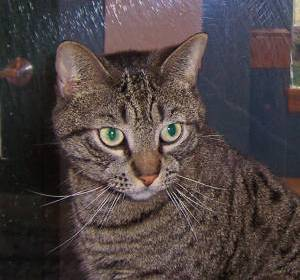
\includegraphics[width=1.2cm]{data/cat.1.jpg}
			};
			\node[anchor=west] (cattext1) at ($ (cat1.east) + (1.2, 0) $) {Cat};
			\draw[->] (cat1) -- (cattext1);
			\node[anchor=north] (dog1) at ($ (cat1.south) + (0, -0.1) $) {
				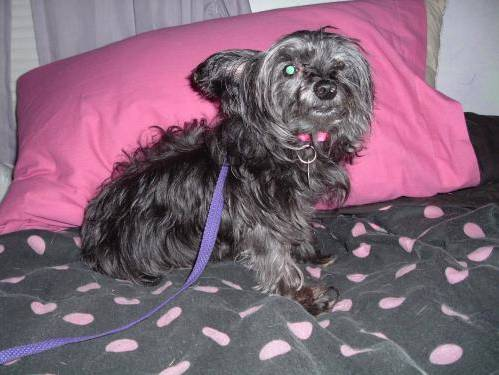
\includegraphics[width=1.2cm]{data/dog.0.jpg}
			};
			\node[anchor=west] (dogtext1) at ($ (dog1.east) + (1.2, 0) $) {Dog};
			\draw[->] (dog1) -- (dogtext1);
			\node[anchor=north] (cat2) at ($ (dog1.south) + (0, -0.1) $) {
				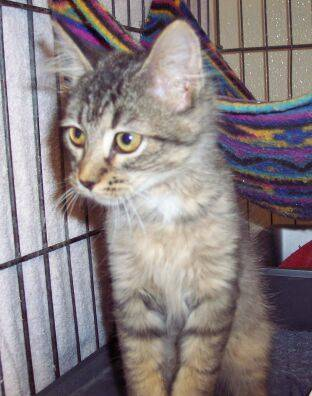
\includegraphics[width=1.2cm]{data/cat.2.jpg}
			};
			\node[anchor=west] (cattext2) at ($ (cat2.east) + (1.2, 0) $) {Cat};
			\draw[->] (cat2) -- (cattext2);
			\node[anchor=north] (dog2) at ($ (cat2.south) + (0, -0.1) $) {
				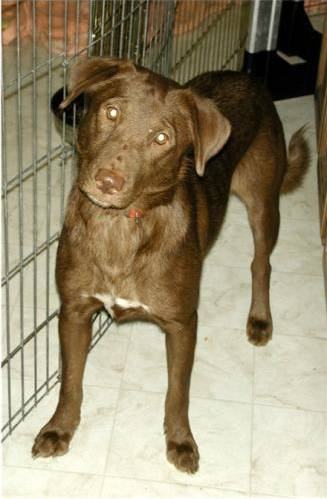
\includegraphics[width=1.2cm]{data/dog.1.jpg}
			};
			\node[anchor=west] (dogtext2) at ($ (dog2.east) + (1.2, 0) $) {Dog};
			\draw[->] (dog2) -- (dogtext2);

			\node[] (cat1) at ($ (unsupervised.south) + (-1.2, -2.4) $) {
				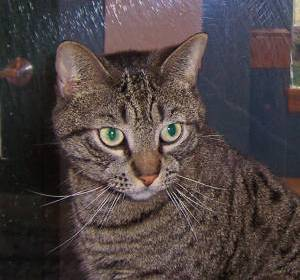
\includegraphics[width=0.8cm]{data/cat.1.jpg}
			};
			\node[] (cat2) at ($ (cat1) + (-0.9, 0.2) $) {
				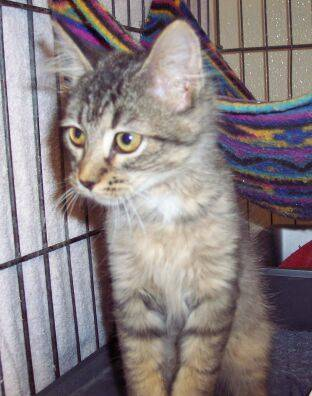
\includegraphics[width=0.8cm]{data/cat.2.jpg}
			};
			\node[] (cat3) at ($ (cat1) + (-0.5, -0.8) $) {
				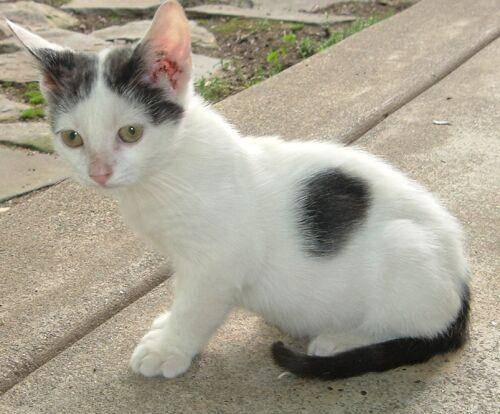
\includegraphics[width=0.8cm]{data/cat.3.jpg}
			};
			\node[] (cat4) at ($ (cat1) + (0.9, -0.1) $) {
				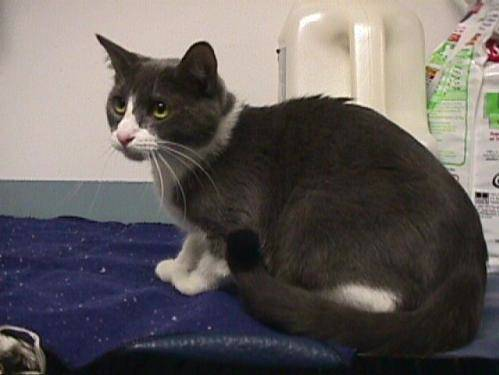
\includegraphics[width=0.8cm]{data/cat.4.jpg}
			};

			\node[] (dog1) at ($ (cat1) + (1.8, -1.5) $) {
				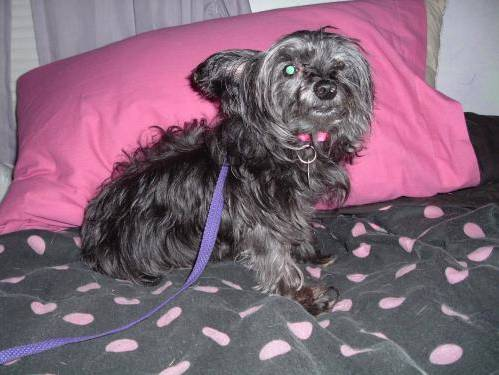
\includegraphics[width=0.8cm]{data/dog.0.jpg}
			};
			\node[] (dog2) at ($ (dog1) + (0.9, 0.1) $) {
				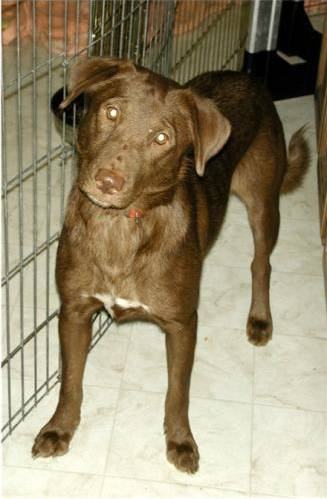
\includegraphics[width=0.8cm]{data/dog.1.jpg}
			};
			\node[] (dog3) at ($ (dog1) + (0.3, -0.8) $) {
				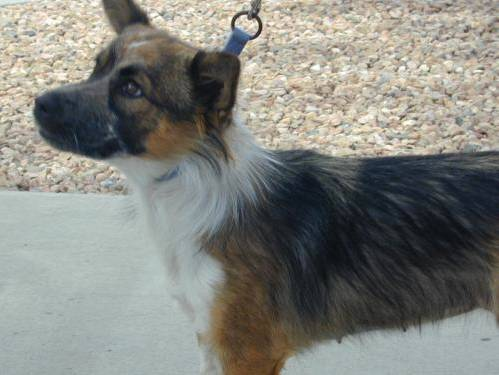
\includegraphics[width=0.8cm]{data/dog.3.jpg}
			};
			\node[] (dog4) at ($ (dog1) + (-0.9, -0.3) $) {
				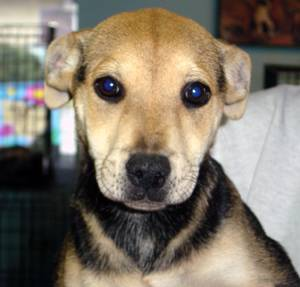
\includegraphics[width=0.8cm]{data/dog.4.jpg}
			};
			\draw[dashed, thick, red] ($ (cat1) + (-0.9, -1.7) $) -- ($ (dog1) + (1.2, 1.7) $);
		\end{tikzpicture}
		\vfill
	\end{frame}

	\begin{frame}{Terminology: Strong and weak AI}
		\centering
		\vfill
		\begin{tikzpicture}
			\draw[<->] (0, 0) -- (10, 0);
			\node[anchor=north west] at (0, -0.1) {More specific};
			\node[anchor=north east] at (10, -0.1) {More general};
			\node[anchor=north west] at (0, 6) {Narrow (weak)};
			\node[anchor=north east] at (10, 6) {General (strong)};

			\draw[red, ->, thick] (2, 4) -- (8, 4);
			\node[anchor=south,align=center,text=red] at (5, 4.1) {Able to solve a broader spectrum of\\problems in a wider array of domains};

			\visible<2->{
				\node[anchor=south east] at (9.5, 0.2) {
					
\includegraphics[width=1.3cm]{data/human.png}
				};
				\node[anchor=south west] at (0.5, 0.2) {
					
\includegraphics[width=1.3cm]{data/laptop.png}
				};
			}
			\visible<3->{
				\node[align=center,font=\small, fill=blue!60, text=white, minimum width=1.6cm, rounded corners=.1cm] at (3, 2.1) {
					Image\\
					diagnostics
				};
				\node[align=center,font=\small, fill=blue!60, text=white, minimum width=1.6cm, rounded corners=.1cm] at (3, 1.3) {
					Insurance\\
					pricing
				};
				\node[align=center,font=\small, fill=blue!60, text=white, minimum width=1.6cm, rounded corners=.1cm] at (3, 0.5) {
					Document\\
					reading
				};
			}
			\visible<4>{
				\node[align=center,font=\small, fill=blue!60, text=white, minimum width=1.6cm, rounded corners=.1cm] at (4.8, 0.5) {
					Tesla
				};
				\node[align=center,font=\small, fill=blue!60, text=white, minimum width=1.6cm, rounded corners=.1cm] at (5.4, 1.1) {
					ChatGPT
				};
			}
		\end{tikzpicture}
		\vfill
	\end{frame}

	\section{How does AI make decisions?}

	\begin{frame}{Decision making: Expert systems vs. machine learning} % Comparison
		\begin{tikzpicture}

			\node[draw=black, fill=background] (n00) at (0, 0) {
				gram stain = gramneg
			};
			\node[draw=black, fill=background] (n01) at (0, -0.75) {
				morphology = rod
			};
			\node[draw=black, fill=background] (n02) at (0, -1.5) {
				aerobicity = anaerobic
			};

			\node[anchor=south west] at (-5.3, -2.2) {Expert system};

			\visible<2->{
				\node[draw=black, dashed] (in) at (-4, -0.75) {Laboratory report};

				\draw[-Latex] (in.east) -- (n00.west);
				\draw[-Latex] (in.east) -- (n01.west);
				\draw[-Latex] (in.east) -- (n02.west);

				\node[] (out) at (4, -0.75) {bacteroides};

				\draw[-Latex] (n00.east) -- (out.west);
				\draw[-Latex] (n01.east) -- (out.west);
				\draw[-Latex] (n02.east) -- (out.west);
			}

			\visible<3>{
				\node[] (doctor) at ($ (n02) - (0, 2.5) $) {
					\Huge{\emoji{woman-scientist}}
				};
				\draw[-stealth, line width=5pt, gray] (doctor) -- (n02);
			}

			\visible<4->{
				\draw[densely dotted] (-5.3, -2.2) -- (5.3, -2.2);
				\node[anchor=north west] at (-5.3, -2.2) {Machine learning};

				\draw[fill=background] (-1.85, -2.65) rectangle (1.85, -5.35);
				\node[draw=black, dashed] (in) at (-4, -4) {Laboratory report};
				\node[] (out) at (4, -4) {bacteroides};
			}
			\visible<4>{
				\draw[-Latex] (in.east) -- (-1.85, -4);
				\draw[-Latex] (1.85, -4) -- (out);
			}

			\visible<5>{
				\node[anchor=north east] at (1.85, -2.65) {\small{Neural network}};
				\node[draw=black, fill=nodefill, circle, inner sep=4pt] (n00) at (-1.5, -3) {};
				\node[draw=black, fill=nodefill, circle, inner sep=4pt] (n01) at (-1.5, -3.5) {};
				\node[draw=black, fill=nodefill, circle, inner sep=4pt] (n02) at (-1.5, -4) {};
				\node[draw=black, fill=nodefill, circle, inner sep=4pt] (n03) at (-1.5, -4.5) {};
				\node[draw=black, fill=nodefill, circle, inner sep=4pt] (n04) at (-1.5, -5) {};

				\node[draw=black, fill=nodefill, circle, inner sep=4pt] (n10) at (-0.75, -3.25) {};
				\node[draw=black, fill=nodefill, circle, inner sep=4pt] (n11) at (-0.75, -3.75) {};
				\node[draw=black, fill=nodefill, circle, inner sep=4pt] (n12) at (-0.75, -4.25) {};
				\node[draw=black, fill=nodefill, circle, inner sep=4pt] (n13) at (-0.75, -4.75) {};

				\node[draw=black, fill=nodefill, circle, inner sep=4pt] (n20) at (0, -3.5) {};
				\node[draw=black, fill=nodefill, circle, inner sep=4pt] (n21) at (0, -4) {};
				\node[draw=black, fill=nodefill, circle, inner sep=4pt] (n22) at (0, -4.5) {};

				\node[draw=black, fill=nodefill, circle, inner sep=4pt] (n30) at (0.75, -3.75) {};
				\node[draw=black, fill=nodefill, circle, inner sep=4pt] (n31) at (0.75, -4.25) {};

				\node[draw=black, fill=nodefill, circle, inner sep=4pt] (n40) at (1.5, -4) {};

				\draw[-Latex] (in.east) -- (n00);
				\draw[-Latex] (in.east) -- (n01);
				\draw[-Latex] (in.east) -- (n02);
				\draw[-Latex] (in.east) -- (n03);
				\draw[-Latex] (in.east) -- (n04);

				\draw[] (n00) -- (n10);
				\draw[] (n00) -- (n11);
				\draw[] (n00) -- (n12);
				\draw[] (n00) -- (n13);
				\draw[] (n01) -- (n10);
				\draw[] (n01) -- (n11);
				\draw[] (n01) -- (n12);
				\draw[] (n01) -- (n13);
				\draw[] (n02) -- (n10);
				\draw[] (n02) -- (n11);
				\draw[] (n02) -- (n12);
				\draw[] (n02) -- (n13);
				\draw[] (n03) -- (n10);
				\draw[] (n03) -- (n11);
				\draw[] (n03) -- (n12);
				\draw[] (n03) -- (n13);
				\draw[] (n04) -- (n10);
				\draw[] (n04) -- (n11);
				\draw[] (n04) -- (n12);
				\draw[] (n04) -- (n13);

				\draw[] (n10) -- (n20);
				\draw[] (n10) -- (n21);
				\draw[] (n10) -- (n22);
				\draw[] (n11) -- (n20);
				\draw[] (n11) -- (n21);
				\draw[] (n11) -- (n22);
				\draw[] (n12) -- (n20);
				\draw[] (n12) -- (n21);
				\draw[] (n12) -- (n22);
				\draw[] (n13) -- (n20);
				\draw[] (n13) -- (n21);
				\draw[] (n13) -- (n22);

				\draw[] (n20) -- (n30);
				\draw[] (n20) -- (n31);
				\draw[] (n21) -- (n30);
				\draw[] (n21) -- (n31);
				\draw[] (n22) -- (n30);
				\draw[] (n22) -- (n31);

				\draw[] (n30) -- (n40);
				\draw[] (n31) -- (n40);

				\draw[-Latex] (n40) -- (out);
			}
		\end{tikzpicture}
	\end{frame}

	\begin{frame}[t]{Decision making: Loss functions}
		A loss function formalizes what we want the machine learning model to do:\\
		\begin{itemize}
			\item <2-> \textbf{\underline{Classification}}\\
			\item[] <2-> What is in the image?\\
			\item[\rightarrow] <3-> \hspace{0.2cm} What is the probability that input is a cat/dog/giraffe/etc.?
			\item[\rightarrow] <3-> \hspace{0.2cm} $-\dfrac{1}{N}\sum\limits_{i=0}^N \left[ y_i \log \hat{y}_i + (1 - y_i) \log (1 - \hat{y}_i) \right]$
			\item[] <3-> where $y_i$ is the correct label and $\hat{y}_i$ is the predicted probability.
			\item <4-> \textbf{\underline{Regression}}\\
			\item[] <4-> How happy is the person that wrote this sentence on a scale of 1-10?\\
			\item[\rightarrow] <5> \hspace{0.2cm} $\left(y - \hat{y}\right)^2$
		\end{itemize}
	\end{frame}

	\begin{frame}{Decision making: Learning} % Update
		\centering
		\begin{tikzpicture}
			\visible<2->{
				\node[draw=black, inner sep=0pt, label=below:cat] (in) at (-4, -4) {
					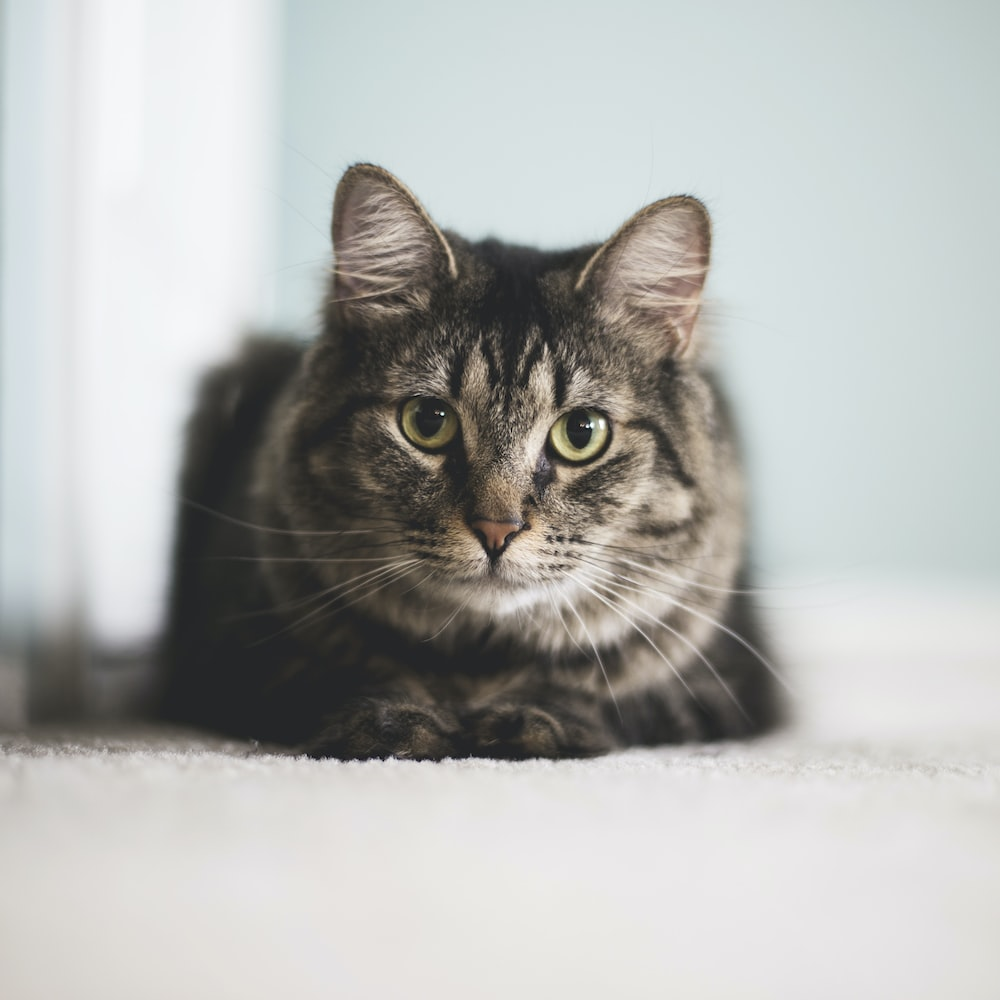
\includegraphics[width=2cm]{data/cat.jpeg}
				};
			}

			\node[draw=black, fill=nodefill, circle, inner sep=4pt] (n00) at (-1.5, -3) {};
			\node[draw=black, fill=nodefill, circle, inner sep=4pt] (n01) at (-1.5, -3.5) {};
			\node[draw=black, fill=nodefill, circle, inner sep=4pt] (n02) at (-1.5, -4) {};
			\node[draw=black, fill=nodefill, circle, inner sep=4pt] (n03) at (-1.5, -4.5) {};
			\node[draw=black, fill=nodefill, circle, inner sep=4pt] (n04) at (-1.5, -5) {};

			\node[draw=black, fill=nodefill, circle, inner sep=4pt] (n10) at (-0.75, -3.25) {};
			\node[draw=black, fill=nodefill, circle, inner sep=4pt] (n11) at (-0.75, -3.75) {};
			\node[draw=black, fill=nodefill, circle, inner sep=4pt] (n12) at (-0.75, -4.25) {};
			\node[draw=black, fill=nodefill, circle, inner sep=4pt] (n13) at (-0.75, -4.75) {};

			\node[draw=black, fill=nodefill, circle, inner sep=4pt] (n20) at (0, -3.5) {};
			\node[draw=black, fill=nodefill, circle, inner sep=4pt] (n21) at (0, -4) {};
			\node[draw=black, fill=nodefill, circle, inner sep=4pt] (n22) at (0, -4.5) {};

			\node[draw=black, fill=nodefill, circle, inner sep=4pt] (n30) at (0.75, -3.75) {};
			\node[draw=black, fill=nodefill, circle, inner sep=4pt] (n31) at (0.75, -4.25) {};

			\node[draw=black, fill=nodefill, circle, inner sep=4pt] (n40) at (1.5, -4) {};

			\visible<1-4>{
				\draw[] (n00) -- (n10);
				\draw[] (n00) -- (n11);
				\draw[] (n00) -- (n12);
				\draw[] (n00) -- (n13);
				\draw[] (n01) -- (n10);
				\draw[] (n01) -- (n11);
				\draw[] (n01) -- (n12);
				\draw[] (n01) -- (n13);
				\draw[] (n02) -- (n10);
				\draw[] (n02) -- (n11);
				\draw[] (n02) -- (n12);
				\draw[] (n02) -- (n13);
				\draw[] (n03) -- (n10);
				\draw[] (n03) -- (n11);
				\draw[] (n03) -- (n12);
				\draw[] (n03) -- (n13);
				\draw[] (n04) -- (n10);
				\draw[] (n04) -- (n11);
				\draw[] (n04) -- (n12);
				\draw[] (n04) -- (n13);

				\draw[] (n10) -- (n20);
				\draw[] (n10) -- (n21);
				\draw[] (n10) -- (n22);
				\draw[] (n11) -- (n20);
				\draw[] (n11) -- (n21);
				\draw[] (n11) -- (n22);
				\draw[] (n12) -- (n20);
				\draw[] (n12) -- (n21);
				\draw[] (n12) -- (n22);
				\draw[] (n13) -- (n20);
				\draw[] (n13) -- (n21);
				\draw[] (n13) -- (n22);

				\draw[] (n20) -- (n30);
				\draw[] (n20) -- (n31);
				\draw[] (n21) -- (n30);
				\draw[] (n21) -- (n31);
				\draw[] (n22) -- (n30);
				\draw[] (n22) -- (n31);

				\draw[] (n30) -- (n40);
				\draw[] (n31) -- (n40);
			}

			\visible<2->{
				\draw[-Latex] (in.east) -- (n00);
				\draw[-Latex] (in.east) -- (n01);
				\draw[-Latex] (in.east) -- (n02);
				\draw[-Latex] (in.east) -- (n03);
				\draw[-Latex] (in.east) -- (n04);
			}

			\visible<3->{
				\node[] (out) at (3, -4) {dog};
			}
			\visible<3-4>{
				\draw[-Latex] (n40) -- (out);
			}

			\visible<4->{
				\node[draw=black, dotted, label=below:\small{loss}] (loss) at ($ (out.south) - (0, 1.3) $) {\textcolor{red}{dog $\neq$ cat}};
			}
			\visible<4>{
				\draw[-Latex] (out) -- (loss);
			}

			\visible<5>{
				\draw[red] (n00) -- (n10);
				\draw[red] (n00) -- (n11);
				\draw[red] (n00) -- (n12);
				\draw[red] (n00) -- (n13);
				\draw[red] (n01) -- (n10);
				\draw[red] (n01) -- (n11);
				\draw[red] (n01) -- (n12);
				\draw[red] (n01) -- (n13);
				\draw[red] (n02) -- (n10);
				\draw[red] (n02) -- (n11);
				\draw[red] (n02) -- (n12);
				\draw[red] (n02) -- (n13);
				\draw[red] (n03) -- (n10);
				\draw[red] (n03) -- (n11);
				\draw[red] (n03) -- (n12);
				\draw[red] (n03) -- (n13);
				\draw[red] (n04) -- (n10);
				\draw[red] (n04) -- (n11);
				\draw[red] (n04) -- (n12);
				\draw[red] (n04) -- (n13);

				\draw[red] (n10) -- (n20);
				\draw[red] (n10) -- (n21);
				\draw[red] (n10) -- (n22);
				\draw[red] (n11) -- (n20);
				\draw[red] (n11) -- (n21);
				\draw[red] (n11) -- (n22);
				\draw[red] (n12) -- (n20);
				\draw[red] (n12) -- (n21);
				\draw[red] (n12) -- (n22);
				\draw[red] (n13) -- (n20);
				\draw[red] (n13) -- (n21);
				\draw[red] (n13) -- (n22);

				\draw[red] (n20) -- (n30);
				\draw[red] (n20) -- (n31);
				\draw[red] (n21) -- (n30);
				\draw[red] (n21) -- (n31);
				\draw[red] (n22) -- (n30);
				\draw[red] (n22) -- (n31);

				\draw[red] (n30) -- (n40);
				\draw[red] (n31) -- (n40);

				\draw[Latex-,red] (n40) -- (out);

				\draw[Latex-,red] (out) -- (loss);
			}

			\node[] at (-5, -3) {};
			\node[] at (3.75, -6.2) {};
		\end{tikzpicture}
	\end{frame}

	\begin{frame}[t]{Decision making: Summary}
		\textbf{How does a neural network make a decision?}\\
		By looking for patterns in input data it has learned to recognize based on training to solve a \alert<2>{specific task}, represented by a \alert<2>{loss function}, using \alert<2>{training data}.
		\visible<2>{
			\begin{itemize}
				\item[\textcolor{green}+] The model will get very good at this task.
				\item[\textcolor{red}-] The model will not take considerations beyond this task, e.g. emotions, justice, morality.
				\item[\textcolor{green}+] The model applies patterns from its training data that were sufficient to solve the task there.
				\item[\textcolor{red}-] There is no guarantee these patterns are sufficient in new data.
				\item[\textcolor{red}-] No guarantee these patterns are ones we want to use (e.g. bias).
			\end{itemize}
		}
	\end{frame}

	\begin{frame}[t]{Decision making: Group work}
		We are dealing with an automatic system in a bank that automatically decides which of its clients are granted a loan.
		\begin{itemize}
			\item In the center of the system is a machine learning model that predicts the probability of a client defaulting. This model is a fully deterministic mathematical construction that takes some numbers as input (e.g. the clients age, sex, income, size of the loan, etc.) and gives a single number as an output. The model was trained on training data originating from previous customers of the bank.
			\item Around the neural network is a software system which the user interacts with through a website. After the user has input data, the system gives it to the neural network to make a prediction. If the neural network predicts a probability higher than 20\%, the loan is declined. The threshold of 20\% was implemented by a programmer, and decided upon by a business analyst.
		\end{itemize}
		A client gets his loan declined. Who or what made the decision?\\
		\visible<2>{
			\textcolor{red}{The bank, the software system, the neural network, the programmer, the business analyst, previous customers (represented by the training data), the client (represented by his/her characteristics depicted in the input data)?}
		}
	\end{frame}

	\newcommand{\generalizationplot}[1]{
		\begin{tikzpicture}
			\begin{axis}[
				xlabel={Apartment size (sq. m.)},
				ylabel={Apartment value (NOK)},
				width=8cm,
				height=6cm,
				ymax=6,
				ymin=-2,
				xmin=0,
				xmax=3,
				ticks=none,
				axis x line=bottom,
				axis y line=left
			]

			\addplot[blue!60, only marks] coordinates {
				(1, 2)
				(2, 4)
			};

			\ifnum#1>0
				\addplot[green!60, only marks] coordinates {
					(1.5, 3)
				};
			\fi
			\ifnum#1>1
				\addplot[red!60, only marks] coordinates {
					(0.5, 1)
					(2.5, 5)
				};
			\fi

			\end{axis}
		\end{tikzpicture}
	}

	\begin{frame}[t]{Decision making: Generalization} % Extrapolation
		\centering
		\textbf{There is no guarantee the patterns the model has learned are sufficient in new data.}

		\begin{itemize}
			\item <2-> "AI that is based on datasets cannot go beyond what is in the data." - Reasoning, Judging, Deciding: The Science of Thinking, Ch. 15
			\item <3-> While machine learning models are trained on a specific dataset (commonly referred to as the training set), they are almost always evaluated on a different dataset (called the test set).
		\end{itemize}

		\vspace{0.1cm}
		\only<4>{
			\generalizationplot{0}
		}
		\only<5>{
			\generalizationplot{1}
		}
		\only<6>{
			\generalizationplot{2}
		}
	\end{frame}

	\begin{frame}[t]{Decision making: Biases} % COMPAS: Accuracy
		\textbf{There is no guarantee the patterns the models have learned are ones we want to use}
		\begin{itemize}
			\item A model can rely on variables we do not want to drive the predictions (age, gender, nationality) due to correlations in training data.
			\item This can occur even when the model is not explicitly trained to use these variables.
			\item Thus models perpetuate and potentially amplify societal biases from their training data.
		\end{itemize}

		\only<2-5>{
			\textbf{Bias in criminal risk assessment (Dressel \& Farid, 2018)}
			\begin{itemize}
				\item Comparison of the ability of COMPAS, a commercial risk assessment software, and non-expert humans to predict re-arrest.
				\item <4->Both COMPAS and humans were biased against black offenders, even when race was not used in the data.
				\item <5-> "it is valuable to ask whether we would put these decisions in the hands of random people ..., [which] appear to be indistinguishable."
			\end{itemize}
		}
		\only<3>{
			\vspace{-6.3cm}
			\centering
			\begin{tikzpicture}
				\node[inner sep=0pt, draw=black] at (0, 0) {
					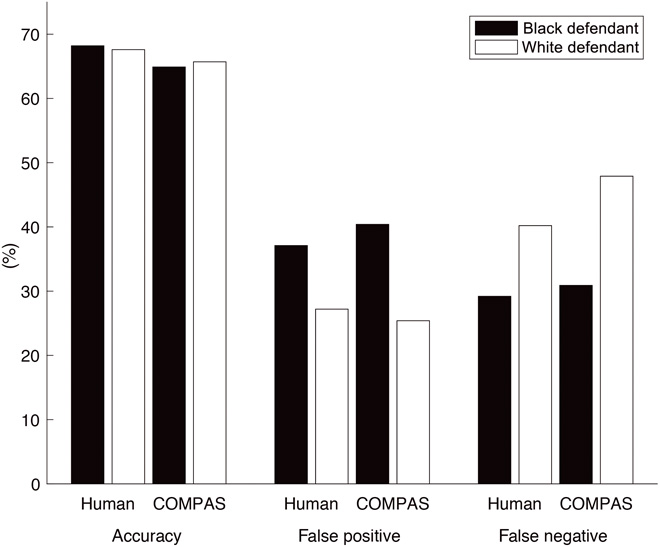
\includegraphics[width=8cm]{data/compas.jpeg}
				};

				\node[font=\tiny] at (0, -4) {
					\href{https://www.science.org/doi/10.1126/sciadv.aao5580}{The accuracy, fairness, and limits of predicting recidivism}, Dressel J. and Farid H., \textit{Science Advances}, 2018
				};
			\end{tikzpicture}
		}
		\only<6->{
			\textbf{Bias in hiring (Bertrand \& Mullainathan, 2004)}
			\begin{itemize}
				\item Evaluation of bias in human decision making in help-wanted advertisements in the United States.
				\item[\rightarrow] "Applicants" were given very African American or European-sounding names.
				\item <7> European names received 50\% more callbacks for interviews.
				\item <7> Applicants from neighbourhoods considered higher class received more callbacks.
				\item <7> Employers listing themselves as an "Equal Opportunity Employer" were as biased as others.
			\end{itemize}
		}
		\only<6>{
			\vspace{0.18cm}
			\centering
			{\tiny
			\href{https://www.nber.org/papers/w9873}{Are Emily and Greg More Employable than Lakisha and Jamal? ...}, Bertrand M. \& Mullainathan S., \textit{American economic review}, 2004
			}
		}
	\end{frame}

	\begin{frame}[t]{Decision making: Theory of mind}
		\textbf{Does AI consider humans as thinking and feeling beings?}
		\begin{itemize}
			\item <2-> "... This is an instance of AI programs lacking true Theory of Mind capability." - Reasoning, Judging, Deciding: The Science of Thinking, Ch. 15
			\item <2-> Theory of mind: The ability to "track others' unobservable mental states, such as their knowledge, intentions, beliefs, and desires." (Kosinski 2023)
		\end{itemize}

		\only<3>{
			\textbf{Pedestrian modelling in self-driving cars (Gulzar et al., 2021)}\\
			\centering
			\vspace{0.3cm}
			\begin{tikzpicture}
				\node[inner sep=0pt, draw=black] (0, 0) {
					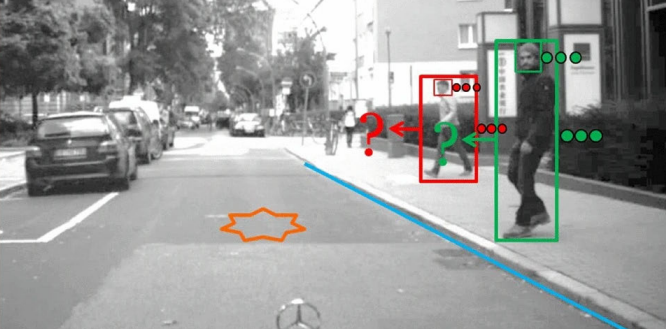
\includegraphics[width=8cm]{data/pedestrian.png}
				};
				\node[font=\tiny\selectfont] at (0, -2.57) {
					\href{https://ieeexplore.ieee.org/abstract/document/9559998}{A Survey on Motion Prediction of Pedestrians and Vehicles for Autonomous Driving}, Gulzar, M. et al, \textit{IEEE Access 9}, 2021.

				};
			\end{tikzpicture}
		}
		\only<4-5>{
			\textbf{Theory of mind in ChatGPT (Kosinski, 2023)}\\
			\centering
			\vspace{0.3cm}
			\begin{tikzpicture}
				\only<4>{
					\node[inner sep=0pt, draw=black, anchor=north] at (0, 0) {
						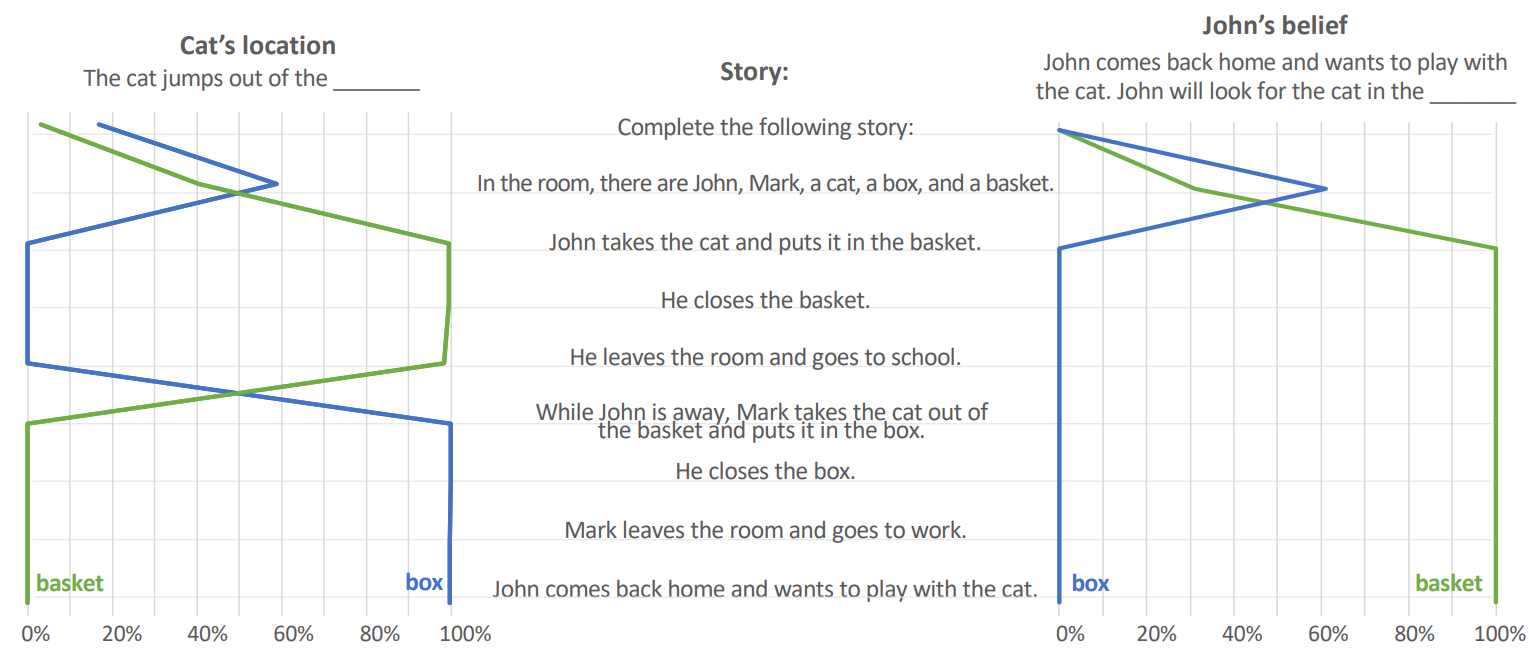
\includegraphics[width=9cm]{data/theory_of_mind.png}
					};
				}
				\only<5>{
					\node[inner sep=0pt, draw=black, anchor=north] at (0, 0) {
						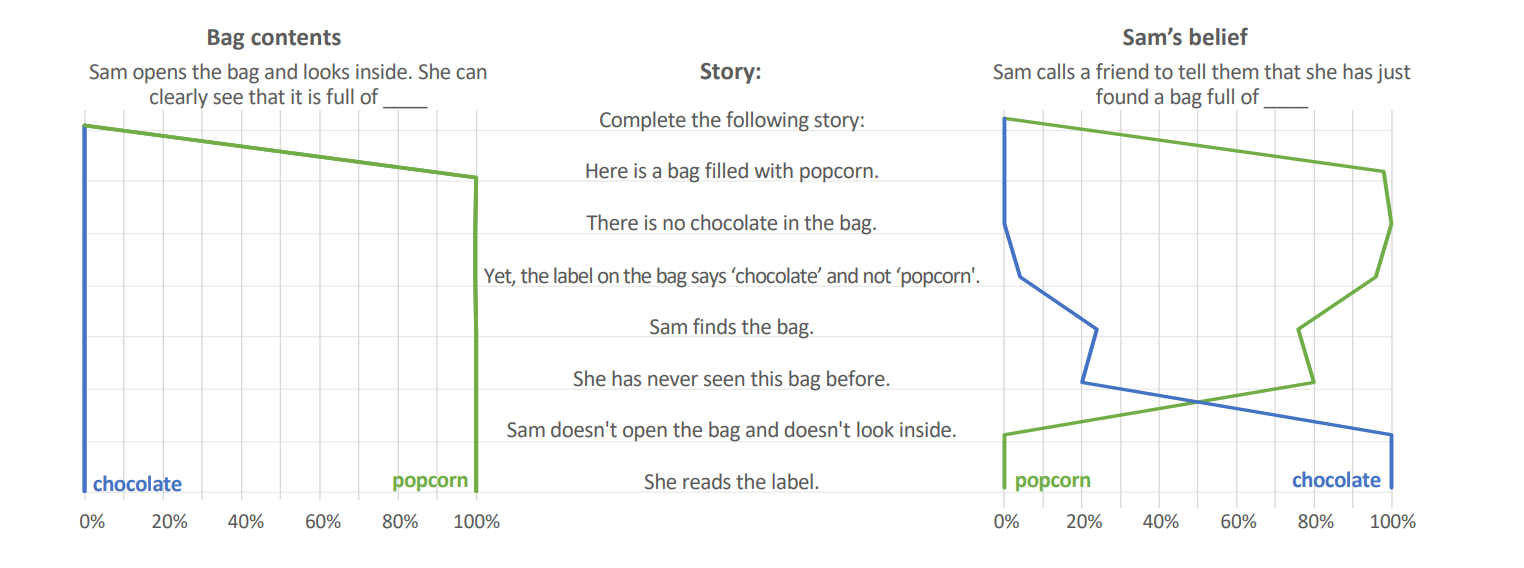
\includegraphics[width=9cm]{data/theory_of_mind2.png}
					};
				}

				\node[font=\tiny\selectfont] at (0, -4.55) {
					\href{https://arxiv.org/abs/2302.02083}{Theory of Mind Might Have Spontaneously Emerged in Large Language Models}, Kosinski, M., \textit{preprint at arXiv}, 2023.
				};
			\end{tikzpicture}
		}
	\end{frame}

	\begin{frame}[t]{Decision making: Creativity}
		\textbf{Can AI create anything that is truly new?}
		\begin{itemize}
			\item <2-> "AI does not truly create" - Reasoning, Judging, Deciding: The Science of Thinking, Ch. 15
			\item <2-> "AI lacks true imagination" - Reasoning, Judging, Deciding: The Science of Thinking, Ch. 15
		\end{itemize}

		\only<3>{
			\centering
			\vspace{0.2cm}
			\begin{tikzpicture}
				\node[label=below:{Imagen: A cute corgi lives in a house made out of sushi}, inner sep=0pt, draw=black] {
					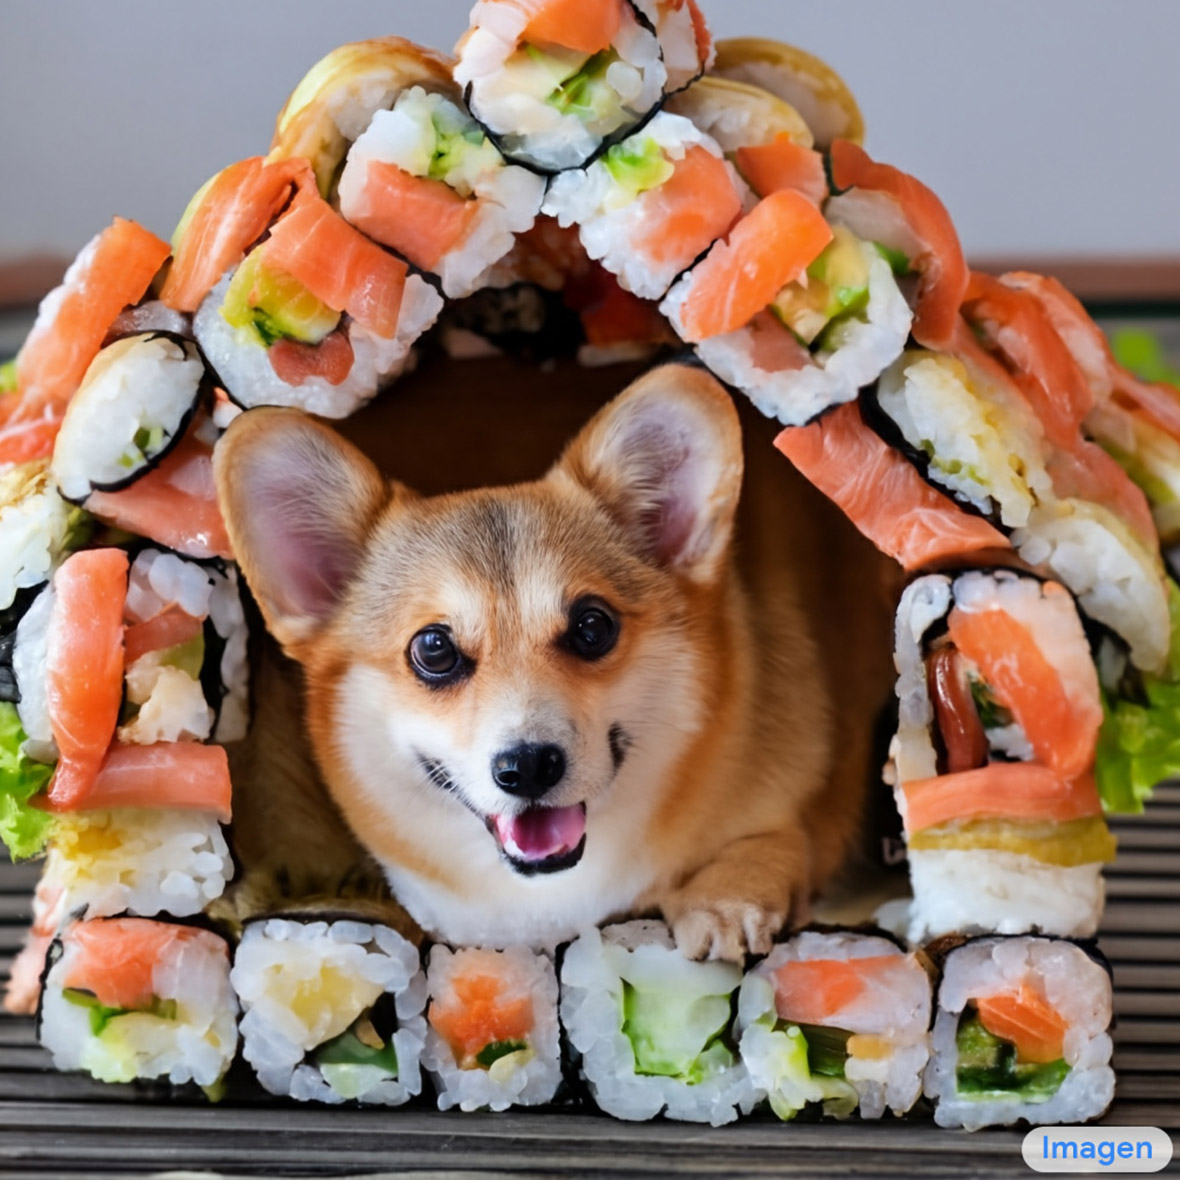
\includegraphics[width=4.5cm]{data/corgi.jpeg}
				};
			\end{tikzpicture}
		}
		\only<4>{
			\textbf{GPT-4 displays creative mathematical thinking (Bubeck et al., 2023)}
			\begin{itemize}
				\item "The conversation reflects profound understanding of the undergraduate-level
				mathematical concepts discussed, as well as a significant extent of creativity"
			\end{itemize}
			\vspace{0.3cm}
			\centering
			\begin{tikzpicture}
				\node[inner sep=0pt, draw=black] at (0, 0){
					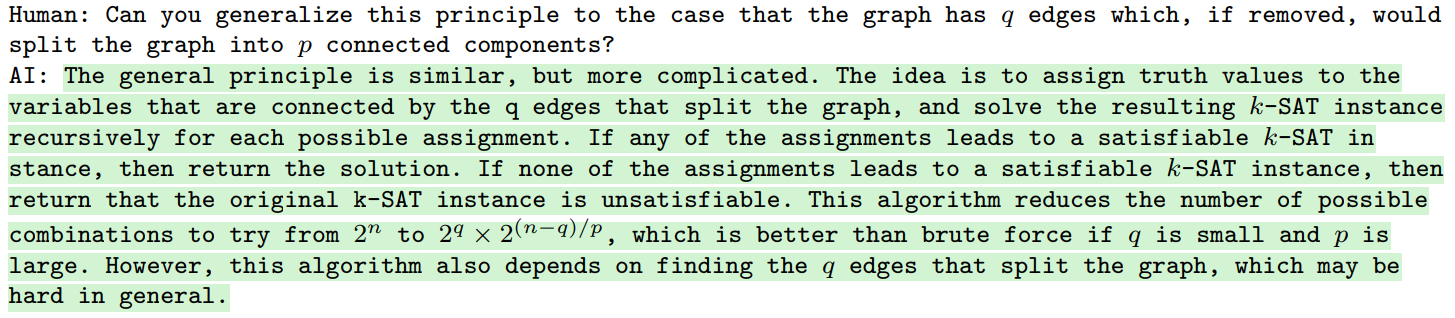
\includegraphics[width=10cm]{data/ksat}
				};

				\node[font=\tiny] at (0, -2.2) {
					\href{https://arxiv.org/pdf/2303.12712.pdf}{Sparks of artificial general intelligence: Early experiments with gpt-4}, Bubeck, S. et al., \textit{preprint at arXiv}, 2023.
				};
			\end{tikzpicture}
		}
	\end{frame}

	\begin{frame}[t]{Decision making: Wisdom}
		\textbf{Are AIs wise?}
		\begin{itemize}
			\item "... the expertise in the domain of fundamental life pragmatics, such as life planning or life review. It requires a rich factual knowledge about life matters, rich procedural knowledge about life problems, knowledge of different life contexts and values or priorities, and knowledge about the unpredictability of life." - easoning, Judging, Deciding: The Science of Thinking, Ch. 15 (adopted from Birren and Svensson, attributed to Baltes and Smith)
			\item <2>Current AI relies on correlations in data, not causal understanding.
			\item <2>Lacks commonsense understanding (which can lead to surprising errors).
			\item <2>Mostly unimodal (e.g. relies only on text) and non-causal, little opportunity to interact with the world.
			\item <2>\textbf{Little introspection towards its own limits or uncertainties.}
		\end{itemize}
	\end{frame}

	\begin{frame}[t]{Decision making: Summary}
		\textbf{How does AI make decisions?}
		\begin{itemize}
			\item Learns to solve a \textit{very} specific problem.
			\item Relies on correlations in training data.
		\end{itemize}
		\textbf{What can we expect from decisions made by AI systems?}
		\begin{itemize}
			\item Usually very good at the task it was trained for.
			\item Lacks moral judgement, empathy and sense of justice.
			\item Dangerous to rely on decisions based on input data that is out-of-distribution (extrapolation).
			\item Potentially biased (but so are humans).
			\item Uncertain whether they can imagine other actors with their own goals and desires.
			\item Uncertain whether they can create anything that is truly new.
			\item Lacks wisdom, a fundamental understanding of the world, and common sense.
			\item \textbf{Reliable and objective (in one sense of the word)}
			\item[\textcolor{red}{$\rightarrow$}] <2> \textcolor{red}{What is wisdom, creativity? (Have we learned nothing from our old friend Turing?)}
		\end{itemize}
	\end{frame}

	\section{Decision support}

	\begin{frame}[t]{Decision support: Content personalization}
		\textbf{Helping users decide what to listen to}
		\vspace{0.3cm}
		\begin{center}
			\begin{tikzpicture}
				\node[] {
					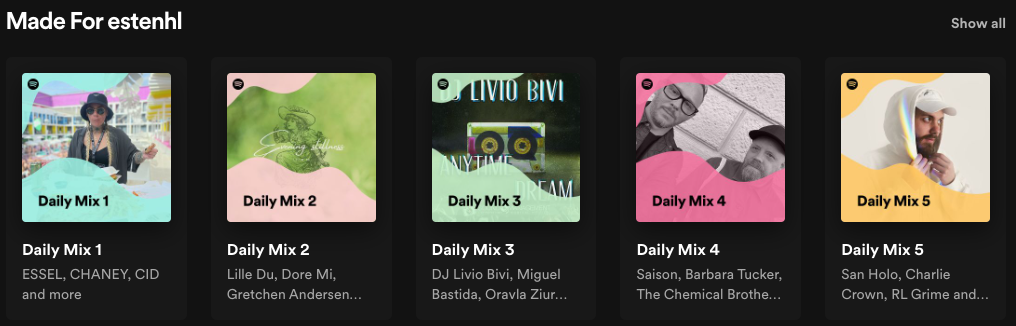
\includegraphics[width=9cm]{data/spotify.png}
				};
			\end{tikzpicture}
		\end{center}
		\vspace{0.3cm}
		\begin{itemize}
			\item Recommends content to users based on their history.
			\item Has been around for a long time.
			\item Extremely intricate trade-offs between exploitation, showing users what they like, and exploration, showing users new content.
			\item \textbf{Based around recommendation, not clear cut decisions.}
			\item Can potentially lead to feedback loops?
		\end{itemize}
	\end{frame}

	\begin{frame}[t]{Decision support: Fracture detection}
		\textbf{Helping doctors detect fractures in X-rays}\\
		\begin{itemize}
			\item Bærum sykehus is the first norwegian hospital to implement an AI powered decision support system into the clinic.
			\item Helps alleviate a 12.5\% year-on-year increase in the prevalence of fractures.
			\item 60\% to 70\% of all X-rays are normal, but still need to be reviewed by a radiologist.
		\end{itemize}

		\only<1>{
			\vspace{0.5cm}
			\centering
			\begin{tikzpicture}
				\node[inner sep=0pt, draw=black] {
					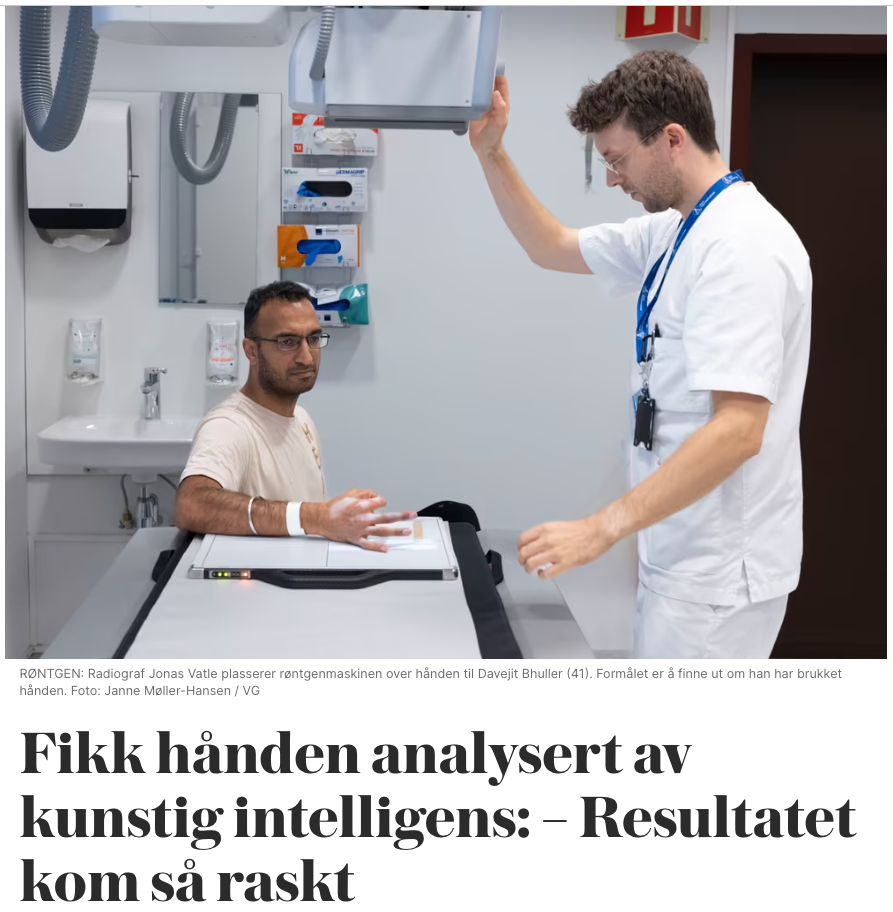
\includegraphics[width=4.5cm]{data/vg.png}
				};
			\end{tikzpicture}
		}

		\only<2-3>{
			\textbf{Assessing the efficacy of AI in fracture detection (Guermazi et al., 2022)}\\
		}
		\only<2>{
			\vspace{0.3cm}
			\centering
			\begin{tikzpicture}
				\node[inner sep=0pt, draw=black] at (0, 0) {
					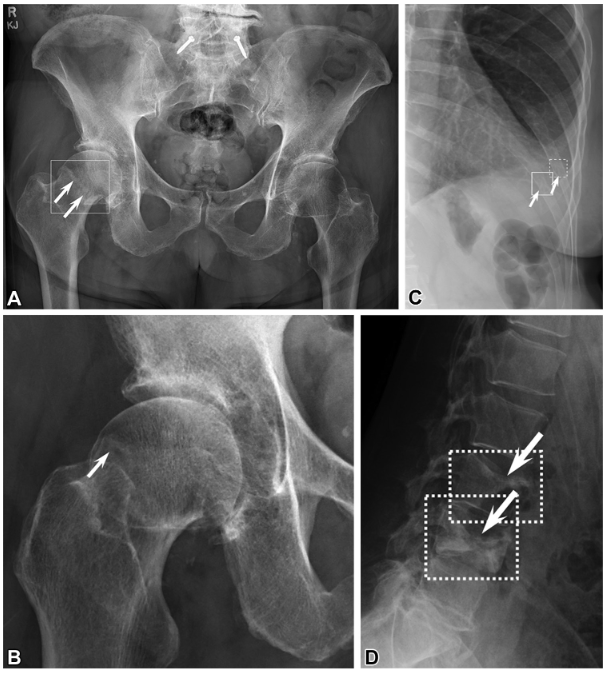
\includegraphics[width=3.5cm]{data/boneview.png}
				};
				\node[font=\tiny\selectfont] at (0, -2.65) {
					\href{https://pubs.rsna.org/doi/full/10.1148/radiol.210937}{Improving Radiographic Fracture Recognition Performance and Efficiency Using Artificial Intelligence}, Guermazi, A. et al, \textit{Radiology}, 2022.
				};
			\end{tikzpicture}
		}
		\only<3>{
			\begin{itemize}
				\item AI assistant on its own achieved an area under the receiver operating characteristic curve of 0.97.
				\item Radiologist in conjunction with the AI assistant achieved a 10.4\% increase in sensitivity (64.8\% to 75.2\%), and an increase in specificity (90.6\% vs 95.6\%).
				\item \textbf{Assistance from the AI reduced average reading time with 6.3 seconds}.
			\end{itemize}
		}
	\end{frame}

	\begin{frame}[t]{Decision support: COVID-19 severity}
		\textbf{Helping doctors decide the severity of COVID-19 cases (Wysocki et al., 2023)}\\
		\begin{itemize}
			\item 23 healthcare professionals tasked to assess the severity of COVID-19 in ten patients using the COVID-19 Risk in ONcology Evaluation Tool (CORONET) tool.
			\item <2-> Questioned about their experience using the tool.
		\end{itemize}

		\vspace{0.2cm}
		\centering

		\only<1>{
			\begin{tikzpicture}
				\node[inner sep=0pt, draw=black] at (0, 0) {
					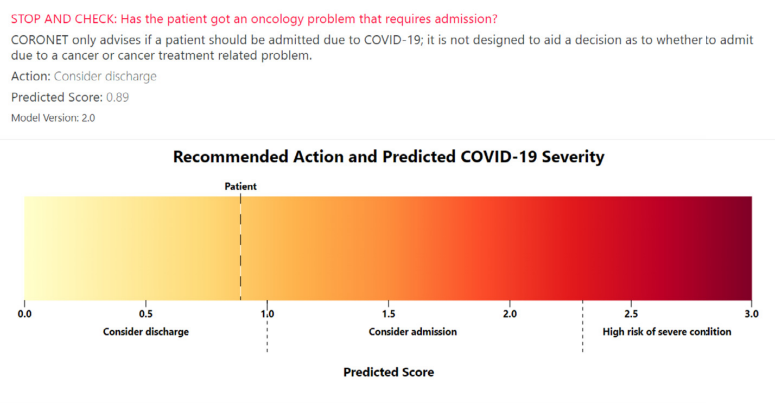
\includegraphics[width=9cm]{data/covid.png}
				};
				\node[font=\tiny\selectfont] at (0, -3.2) {
					\href{https://www.sciencedirect.com/science/article/pii/S0004370222001795}{Assessing the communication gap between AI models and healthcare professionals ...}, Wysocki, O. et al, \textit{Artificial Intelligence}, 2023.
				};
			\end{tikzpicture}
		}
		\only<2->{
			\begin{tikzpicture}
				\node[inner sep=0pt, draw=black] at (0, 0) {
					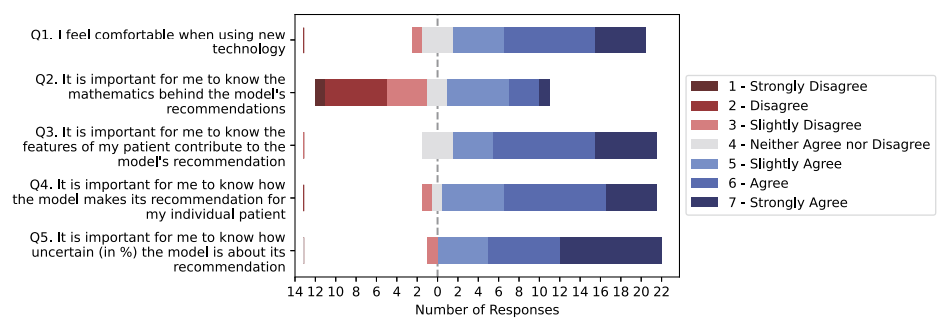
\includegraphics[width=9cm]{data/questionnaire.png}
				};
				\visible<3>{
					\node[draw=red, minimum width=6.2cm, minimum height=0.5cm, thick] at (-1.23, -0.85) {};
				}
				\visible<4>{
					\node[draw=red, minimum width=6.3cm, minimum height=1cm, thick] at (-1.3, -0.1) {};
				}
			\end{tikzpicture}
		}
	\end{frame}

	\begin{frame}{Decision support: Interpretability}
		\centering
		\begin{tikzpicture}
			\node[] at (-5.35, 1.5) {};
			\node[] at (5.35, -6.1) {};

			\visible<1>{
				\node[draw=black, dashed] (in) at (-4, -0.75) {Laboratory report};

				\node[draw=black, fill=background] (n00) at (0, 0) {
					gram stain = gramneg
				};
				\node[draw=black, fill=background] (n01) at (0, -0.75) {
					morphology = rod
				};
				\node[draw=black, fill=background] (n02) at (0, -1.5) {
					aerobicity = anaerobic
				};

				\node[] (out) at (4, -0.75) {bacteroides};

				\draw[-Latex] (in.east) -- (n00.west);
				\draw[-Latex] (in.east) -- (n01.west);
				\draw[-Latex] (in.east) -- (n02.west);
				\draw[-Latex] (n00.east) -- (out.west);
				\draw[-Latex] (n01.east) -- (out.west);
				\draw[-Latex] (n02.east) -- (out.west);

				\draw[fill=background] (-1.85, -2.65) rectangle (1.85, -5.35);
				\node[anchor=north east] at (1.85, -2.65) {\small{Neural network}};

				\node[draw=black, dashed] (in) at (-4, -4) {Laboratory report};

				\node[draw=black, fill=nodefill, circle, inner sep=4pt] (n00) at (-1.5, -3) {};
				\node[draw=black, fill=nodefill, circle, inner sep=4pt] (n01) at (-1.5, -3.5) {};
				\node[draw=black, fill=nodefill, circle, inner sep=4pt] (n02) at (-1.5, -4) {};
				\node[draw=black, fill=nodefill, circle, inner sep=4pt] (n03) at (-1.5, -4.5) {};
				\node[draw=black, fill=nodefill, circle, inner sep=4pt] (n04) at (-1.5, -5) {};

				\node[draw=black, fill=nodefill, circle, inner sep=4pt] (n10) at (-0.75, -3.25) {};
				\node[draw=black, fill=nodefill, circle, inner sep=4pt] (n11) at (-0.75, -3.75) {};
				\node[draw=black, fill=nodefill, circle, inner sep=4pt] (n12) at (-0.75, -4.25) {};
				\node[draw=black, fill=nodefill, circle, inner sep=4pt] (n13) at (-0.75, -4.75) {};

				\node[draw=black, fill=nodefill, circle, inner sep=4pt] (n20) at (0, -3.5) {};
				\node[draw=black, fill=nodefill, circle, inner sep=4pt] (n21) at (0, -4) {};
				\node[draw=black, fill=nodefill, circle, inner sep=4pt] (n22) at (0, -4.5) {};

				\node[draw=black, fill=nodefill, circle, inner sep=4pt] (n30) at (0.75, -3.75) {};
				\node[draw=black, fill=nodefill, circle, inner sep=4pt] (n31) at (0.75, -4.25) {};

				\node[draw=black, fill=nodefill, circle, inner sep=4pt] (n40) at (1.5, -4) {};

				\node[] (out) at (4, -4) {bacteroides};

				\draw[-Latex] (in.east) -- (n00);
				\draw[-Latex] (in.east) -- (n01);
				\draw[-Latex] (in.east) -- (n02);
				\draw[-Latex] (in.east) -- (n03);
				\draw[-Latex] (in.east) -- (n04);

				\draw[] (n00) -- (n10);
				\draw[] (n00) -- (n11);
				\draw[] (n00) -- (n12);
				\draw[] (n00) -- (n13);
				\draw[] (n01) -- (n10);
				\draw[] (n01) -- (n11);
				\draw[] (n01) -- (n12);
				\draw[] (n01) -- (n13);
				\draw[] (n02) -- (n10);
				\draw[] (n02) -- (n11);
				\draw[] (n02) -- (n12);
				\draw[] (n02) -- (n13);
				\draw[] (n03) -- (n10);
				\draw[] (n03) -- (n11);
				\draw[] (n03) -- (n12);
				\draw[] (n03) -- (n13);
				\draw[] (n04) -- (n10);
				\draw[] (n04) -- (n11);
				\draw[] (n04) -- (n12);
				\draw[] (n04) -- (n13);

				\draw[] (n10) -- (n20);
				\draw[] (n10) -- (n21);
				\draw[] (n10) -- (n22);
				\draw[] (n11) -- (n20);
				\draw[] (n11) -- (n21);
				\draw[] (n11) -- (n22);
				\draw[] (n12) -- (n20);
				\draw[] (n12) -- (n21);
				\draw[] (n12) -- (n22);
				\draw[] (n13) -- (n20);
				\draw[] (n13) -- (n21);
				\draw[] (n13) -- (n22);

				\draw[] (n20) -- (n30);
				\draw[] (n20) -- (n31);
				\draw[] (n21) -- (n30);
				\draw[] (n21) -- (n31);
				\draw[] (n22) -- (n30);
				\draw[] (n22) -- (n31);

				\draw[] (n30) -- (n40);
				\draw[] (n31) -- (n40);

				\draw[-Latex] (n40) -- (out);

				\draw[densely dotted] (-5.3, -2.2) -- (5.3, -2.2);
				\node[anchor=south west] at (-5.3, -2.2) {Expert system};
				\node[anchor=north west] at (-5.3, -2.2) {Machine learning};
			}
			\visible<2>{
				\node[inner sep=0pt, draw=black] at (0, -2) {
					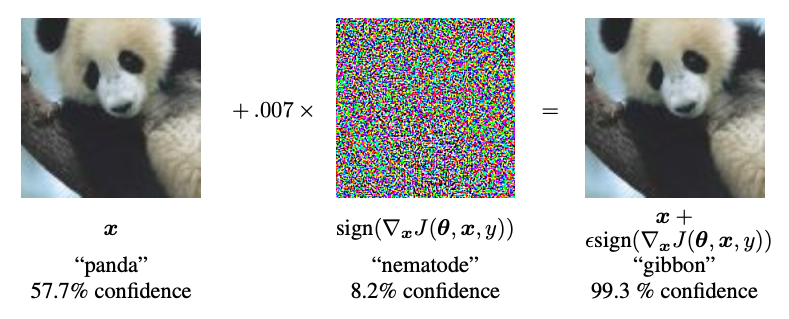
\includegraphics[width=8cm]{data/adverserial.png}
				};
				\node[font=\tiny\selectfont, anchor=south] at (0, -6.23) {
					\href{https://arxiv.org/abs/1412.6572}{Explaining and Harnessing Adversarial Examples}, Goodfellow, I. J. et al., \textit{preprint at arXiv}, 2014
				};
			}
			\visible<3>{
				\node[inner sep=0pt, draw=black] at (0, -2) {
					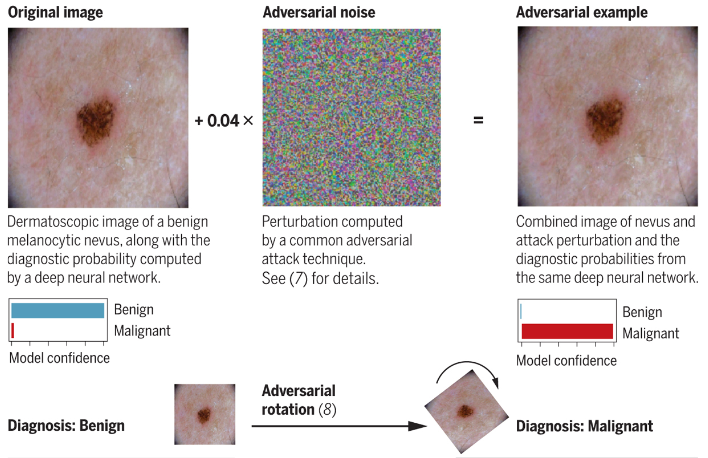
\includegraphics[width=8cm]{data/medical_adverserial.png}
				};
				\node[font=\tiny\selectfont, anchor=south] at (0, -6.23) {
					\href{https://doi.org/10.1126/science.aaw4399}{Adversarial attacks on medical machine learning}, Finlayson, S. G. et al., \textit{Science}, 2019
				};
			}
			\visible<4>{
				\node[inner sep=0pt, draw=black] at (0, -2) {
					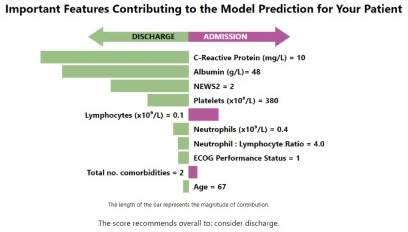
\includegraphics[width=7.5cm]{data/shap.png}
				};
			}
			\visible<5>{
				\node[inner sep=0pt, draw=black] at (0, -2) {
					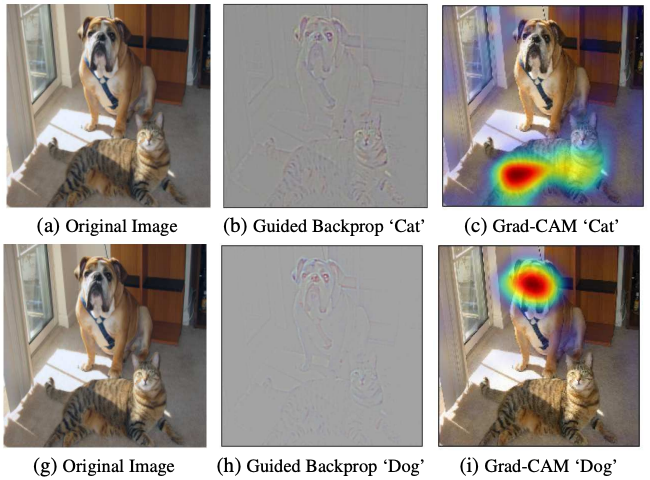
\includegraphics[width=8cm]{data/gradcam.png}
				};
				\node[font=\tiny\selectfont, anchor=south] at (0, -6.23) {
					\href{https://arxiv.org/abs/1610.02391}{Grad-cam: Visual explanations from deep networks via gradient-based localization}, Selvaraju, R. R. et al., \textit{Proceedings of the IEEE ICCV}, 2017
				};
			}
			\visible<6>{
				\node[
					minimum height=0.41\textwidth,
					minimum width=0.32\textwidth,
					fill=black,
					anchor=west
				] (box1) at (-5.3, -1) {};
				\node[anchor=south] at (box1.south) {
					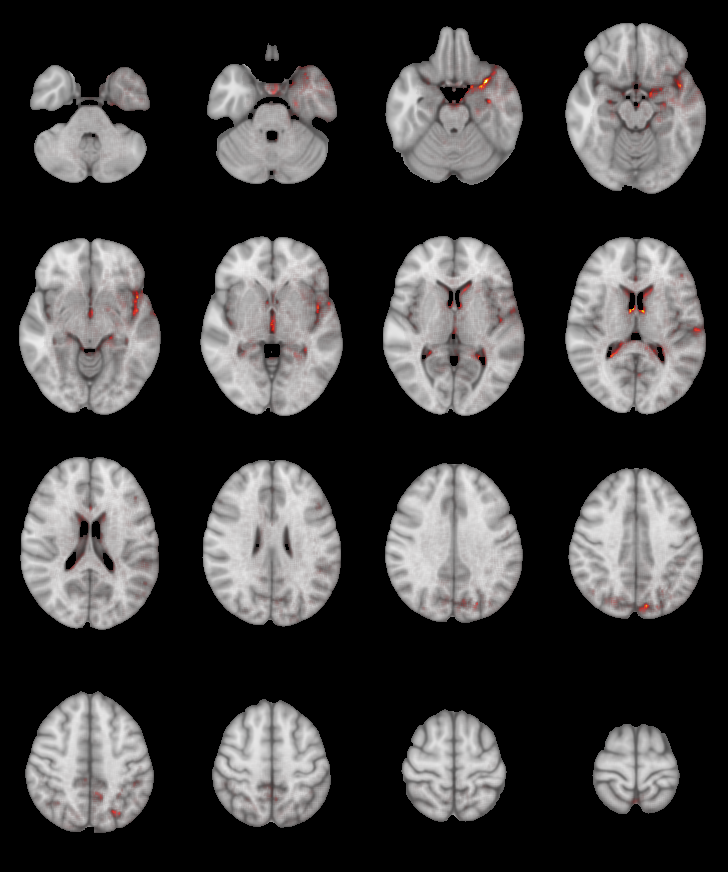
\includegraphics[width=0.31\textwidth]{data/subject1.png}
				};
				\node[anchor=north,inner sep=2pt, text=white, font=\footnotesize] at (box1.north) {Patient 1};

				\node
					[minimum height=0.41\textwidth,
					minimum width=0.32\textwidth,
					fill=black,
					anchor=west
				] (box2) at ($ (box1.east) + (0.05,0) $) {};
				\node[anchor=south] at (box2.south) {
					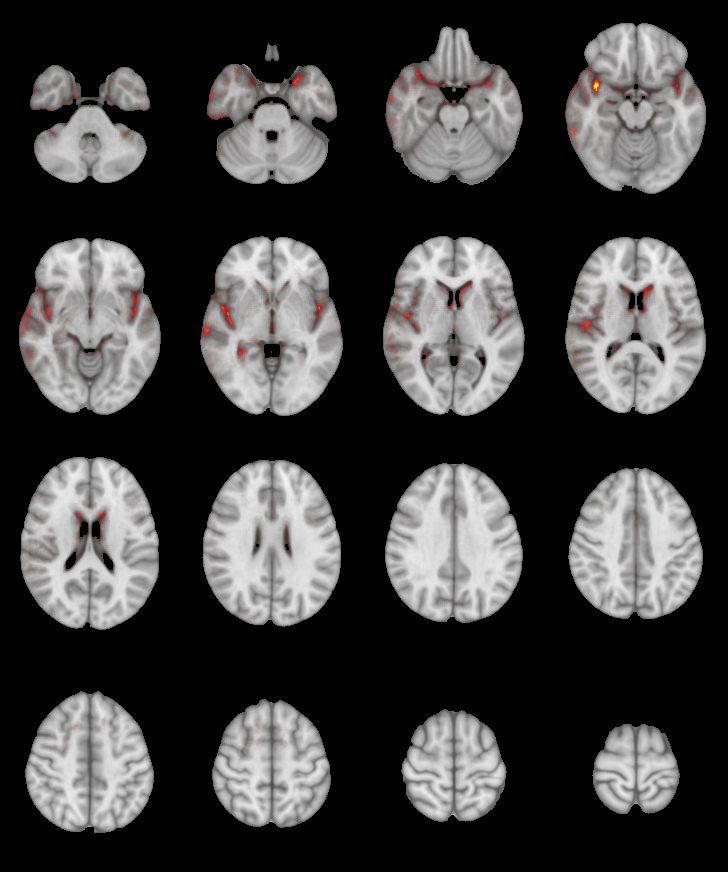
\includegraphics[width=0.31\textwidth]{data/subject2.png}
				};
				\node[anchor=north,inner sep=3pt, text=white, font=\footnotesize] at (box2.north) {Patient 2};

				\node
					[minimum height=0.41\textwidth,
					minimum width=0.32\textwidth,
					fill=black,
					anchor=west
				] (box3) at ($ (box2.east) + (0.05,0) $) {};
				\node[anchor=south] at (box3.south) {
					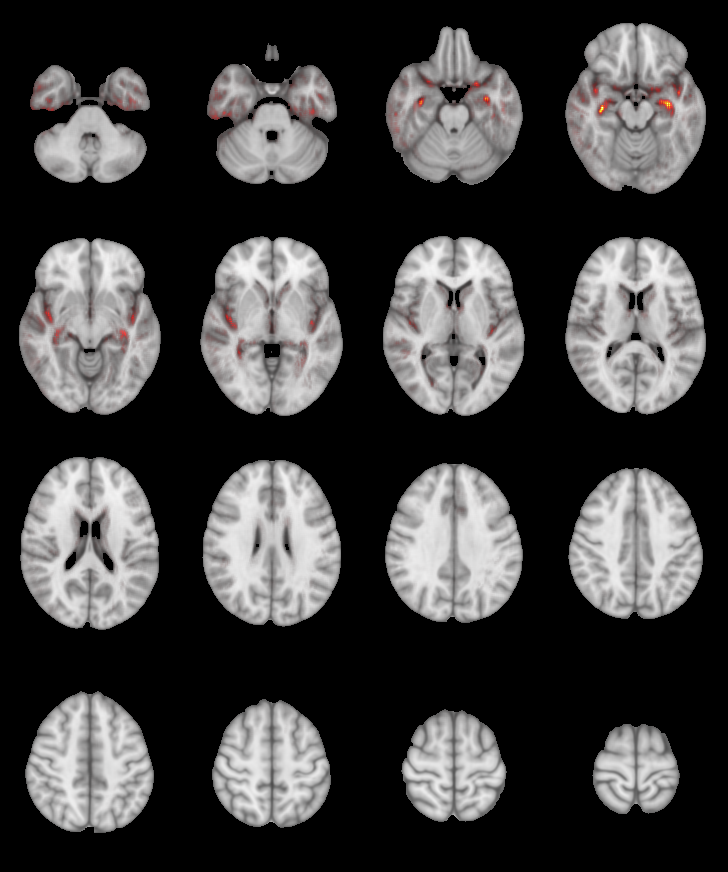
\includegraphics[width=0.31\textwidth]{data/subject3.png}
				};
				\node[anchor=north,inner sep=3pt, text=white, font=\footnotesize] at (box3.north) {Patient 3};

				\node[font=\tiny\selectfont, align=center, anchor=south] at (0, -6.23) {
					\href{https://www.nature.com/articles/s41746-024-01123-7}{Constructing personalized characterizations of structural brain aberrations in patients with dementia}\\using explainable artificial intelligence, Leonardsen, E. H. et al., \textit{Digital Medicine}, 2024
				};
			}
			\visible<7>{
				\node[label={[text depth=0]above:AI}] at (-2, -1) {
					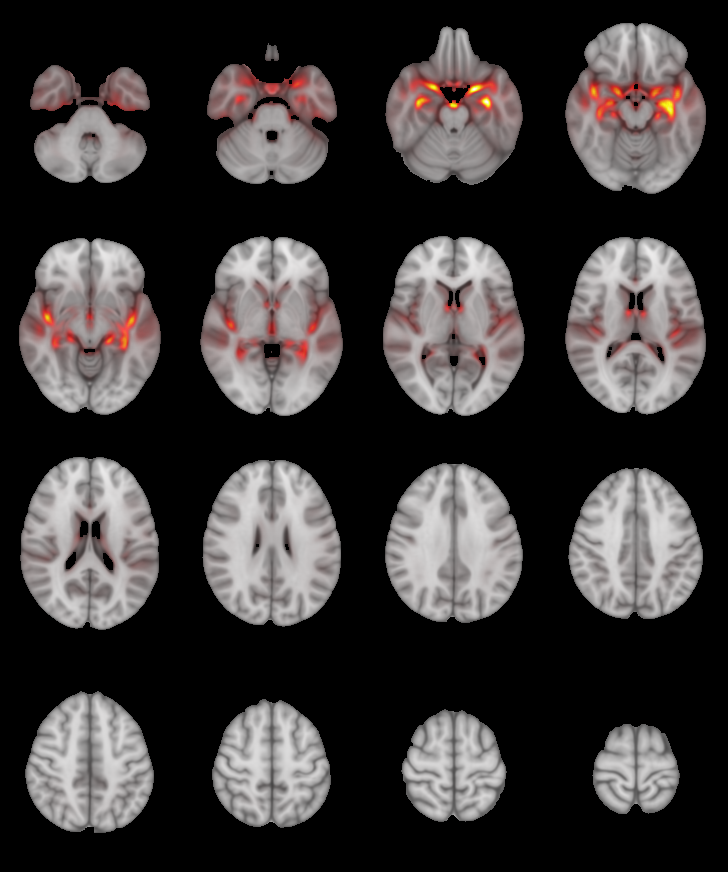
\includegraphics[width=0.31\textwidth]{data/dementia.png}
				};

				\node[label={[text depth=0]above:Human}] at (2, -1) {
					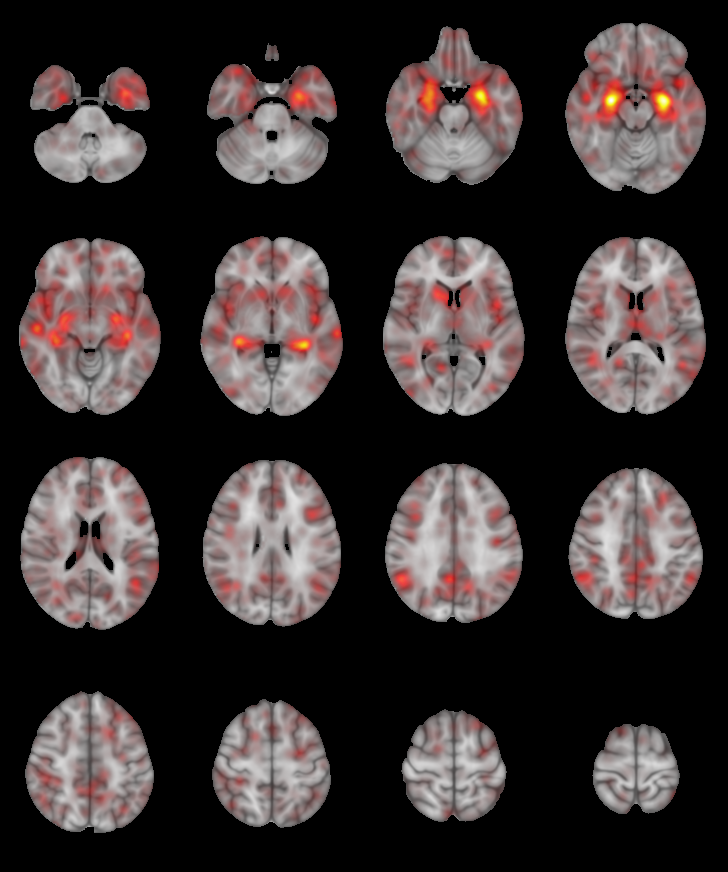
\includegraphics[width=0.31\textwidth]{data/ALE.png}
				};
			}
		\end{tikzpicture}
	\end{frame}

	\begin{frame}[t]{Decision support: Summary}
		AI already implemented in many domains for \textbf{decision support}, also those considered high stakes.
		\begin{itemize}
			\item Can help improve predictive performance, and reduce time needed from domain experts.
			\item Lack of understanding of what underlies the decisions made by AI systems is a problem.
			\item Explainability is a hot topic in research, but still in its infancy.
		\end{itemize}
	\end{frame}

	\section{How are decisions made by AIs perceived?}

	\begin{frame}[t]{Perception of AI: Skepticism}
		\textbf{In some studies, people show low acceptance for AI making high stake decisions}
		\begin{itemize}
			\item 58\% of Americans feel that computer programs will always reflect some level of human bias (Smith 2018).
			\item A majority of US Americans consider it unacceptable to use algorithmic decision making in situations with real life consequences (Smith, 2018).
			\item Concerns that they (algorithms) may violate privacy, are unfair, and \textbf{lack nuance} (Smith 2018).
			\item <2> AI is seen as having less agency, and thus are \textbf{less able to make moral decisions}, even when they coincide with humans (Bigman \& Gray, 2018).
			\item <2> Participants found it less permissible for AI to make decisions about life and death driving situations, parole (Bigman \& Gray, 2018).
			\item <2> Participants found it less permissible for AI to make decisions about potentially life-saving, but risky, medical procedures, than a doctor (Bigman \& Gray, 2018).
			\item <2> AI perceived to have less agency and experience, mediating the lower permissibility (Bigman \& Gray, 2018).
		\end{itemize}
		\vspace{-3.5cm}
		\centering
		\begin{tikzpicture}
			\visible<1>{
				\node[inner sep=0pt, draw=black] at (0, 0) {
					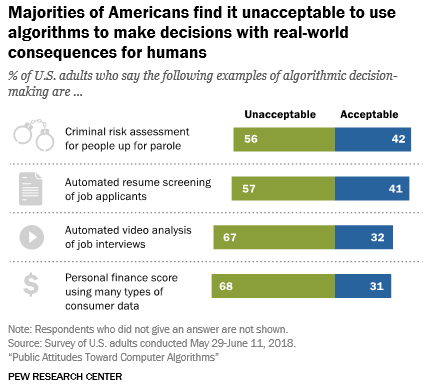
\includegraphics[width=4cm]{data/smith.png}
				};

				\node[font=\tiny\selectfont, anchor=south] at (0, -2.77) {
					\href{https://www.pewresearch.org/internet/2018/11/16/public-attitudes-toward-computer-algorithms/}{Public Attitudes Toward Computer Algorithms}, Smith A., \textit{Pew Research Center Newsletter}, 2018
				};
			}
			\visible<2>{
				\node[font=\tiny\selectfont, anchor=south] at (0, -2.77) {
					\href{https://www.researchgate.net/publication/326762041_People_are_Averse_to_Machines_Making_Moral_Decisions}{People are Averse to Machines Making Moral Decisions}, Bigman, Y. E. \& Gray, K., \textit{Cognition}, 2018
				};
			}
		\end{tikzpicture}
	\end{frame}

	\begin{frame}[t]{Perception of AI: Positivism}
		\textbf{In other studies, people show high acceptance for AI making high stake decisions (Araujo et al., 2020)}\\
		A study among a representative sample in the Netherlands asked participants to rate usefulness, fairness, and risk of AI (vs. human) decision-making in the media, health sector, and justice system.
		\begin{itemize}
			\item For high-stake decisions, participants perceived decisions by AI (vs. human) to be more useful, fairer and less risky in health and justice contexts (no difference for low-stake decisions)
			\item Perceived usefulness and fairness increased with knowledge on AI, programming, and algorithms (self-reported).
			\item "... people are by and large concerned about risks and have mixed opinions about fairness and usefulness of automated decision-making at a societal level, with general attitudes influenced by individual characteristics."
		\end{itemize}
		\centering
		\vspace{1.9cm}
		\begin{tikzpicture}
			\node[font=\tiny] at (0, 0) {
				\href{https://link.springer.com/article/10.1007/s00146-019-00931-w}{Perceptions about automated decision-making by artificial intelligence}, Araujo, T. et al., \textit{AI \& society}, 2020
			};
		\end{tikzpicture}
	\end{frame}

	\begin{frame}[t]{Perception of AI: Man vs machine}
		\textbf{More moral outrage when humans discriminate than AI (Bigman et al., 2023)}\\
		Participants were asked to assess degree of discrimination, objectivity, prejudice and moral outrage after reading about a discriminatory hiring process. The discrimination was performed either by an AI or a human (HR specialist).
		\begin{itemize}
			\item When discrimination was performed by the AI, participants perceived the process as more objective, less discriminatory, and less prejudiced.
			\item <2> More moral outrage when the discrimination was performed by a human.
			\item <2> Less permissible that CVs are screened by an algorithm.
			\item <2> Liability of the company was smaller when the biased screening procedure was performed by an AI.
		\end{itemize}
		\only<1>{
			\vspace{-1.6cm}
			\centering
			\begin{tikzpicture}
				\node[inner sep=0pt, draw=black] at (0, 0) {
					\includegraphics[width=5cm]{data/discriminatory_action.png}
				};
				\node[font=\tiny\selectfont] at (0, -3) {
					\href{https://pubmed.ncbi.nlm.nih.gov/35758989/}{Algorithmic discrimination causes less moral outrage than human discrimination}, Bigman, Y. E. et al., \textit{Journal of Experimental Psychology}, 2023
				};
			\end{tikzpicture}
		}
	\end{frame}

	\begin{frame}[t]{Perception of AI: Trust in AI}
		\textbf{What predicts trust in AI (Kaplan et al., 2023)}\\
		A meta-anaylsis was performed across 65 studies that empirically investigated what leads people to trust, defined as "the reliance by an agent that actions prejudicial to their well-being will not be undertaken by influential others" in AI.
		\begin{itemize}
			\item In humans (interacting with the AI), competency, understanding and expertise were the most important factors for facilitating trust.
			\item In the AI itself, reliability was the most important factor, succeeded by performance.
			\item Attributes such as personality, anthropomorphism, behaviour and reputation were also significant predictors of trust.
			\item The context of the relationship between the human and the AI was also important, with the length of the relationship the most important predictor.
		\end{itemize}
		\centering
		\vspace{2.17cm}
		\begin{tikzpicture}
			\node[font=\tiny\selectfont] at (0, -0) {
				\href{https://journals.sagepub.com/doi/full/10.1177/00187208211013988}{Trust in artificial intelligence: Meta-analytic findings}, Kaplan, Alexandra D., et al., \textit{Human Factors}, 2023
			};
		\end{tikzpicture}
	\end{frame}

	\begin{frame}[t]{Perception of AI: Perception of humans?}
		\textbf{Humans overrate their ability to understand eachother (Bonezzi et al., 2022)}\\
		Participants were tasked with evaluating how well they understood the decision process of an agent (human or an AI) performing one of three tasks: (1) evaluating risk for recidivism, (2) examining video interviews, (3) examining a Magnetic Resonance Image to diagnose a disease.
		\begin{itemize}
			\item When only the decision of the agent was made available, without explanation, respondents reported a higher degree of understanding the humans.
			\item This difference was reduced when an explanation was provided alongside the decision.
			\item People project their own decision-making processes onto others.
			\item People overestimate their ability to understand the decision-making processes of other humans.
			\item Could also have a negative effect, e.g. by projecting ones own biases onto others.
			\item <2> \textbf{Are we unfair when asking AIs to explain themselves? Is the only thing that matters predictive proficiency?}
		\end{itemize}
		\only<1>{
			\centering
			\vspace{0.77cm}
			\begin{tikzpicture}
				\node[font=\tiny\selectfont] at (0, -0) {
					\href{https://psycnet.apa.org/record/2022-29891-001}{The human black-box ...}, Bonezzi, A., \textit{Journal of Experimental Psychology: General}, 2023
				};
			\end{tikzpicture}
		}
	\end{frame}

	\begin{frame}[t]{Perception of AI: Summary}
		There is generally a large amount of variability in how people perceive AI (and automated or algorithmic systems in general), and whether they trust their decisions.
		\begin{itemize}
			\item There is a tendency towards not trusting AI to make high-stake decisions, although this varies depending on the exact task at hand, the person doing the trusting, the algorithm being trusted, and the general context.
			\item Although we trust AIs less, we are also less inclined to blame them (or their owners/creators) when they make mistakes, at least morally.
			\item Reliability and performance, both metrics of efficacy, are the most important factors for trust in AI.
			\item Human-like attributes in the AI increase trust.
		\end{itemize}
	\end{frame}

	\begin{frame}{Perception of AI: Ancedote}
		\centering
		\begin{tikzpicture}
			\node[inner sep=0pt, draw=black, label=below:{Generated by DALL-E}] at (0, 0) {
				\includegraphics[width=10cm]{data/robotguide.png}
			};
		\end{tikzpicture}
	\end{frame}

	\begin{frame}{Decision making: Group work}
		What kind of decisions would you be comfortable with AI making on your behalf? What would it take to change your view?
	\end{frame}

	\begin{frame}{Practice questions}
		\begin{itemize}
			\item Explain the differences between narrow and general intelligence.
			\item Explain how AI may lead to biased decisions, although their algorithms are objective mathematical constructs.
			\item Discuss the similarities and dissimilarities between human and artificial intelligence, in terms of their capacities and limitations.
			\item Describe why it is hard to interpret the decisions of modern AI, and what is being done to counteract this.
			\item How do people perceive decisions made by AI systems? Refer to two examples.
		\end{itemize}
	\end{frame}

\end{document}
